%&latex
\documentclass[12pt,a4paper]{article}
\setlength{\topmargin}{-0.8in}
\setlength{\oddsidemargin}{-4mm}
\setlength{\textwidth}{6.5in}
\setlength{\textheight}{10in}

\usepackage{amstext}
\usepackage{amsmath}
\usepackage{graphicx}
\usepackage{wrapfig}
\usepackage{mathptmx}
\usepackage[normalem]{ulem}
\usepackage{amssymb}
\usepackage{color}
\usepackage{hyperref}
\usepackage{subeqn}
\usepackage{fancyhdr}
\pagestyle{fancy}
\lhead{PH-624}
\rhead{P. Arumugam}



\begin{document} 

\title{PH 624 - Computational Nuclear Structure Physics}
\author{P. Arumugam, Department of Physics, IIT Roorkee}
\maketitle

\section{Hermite polynomials}
Hermite polynomials, $H_n(x)$, have got extensive applications in quantum
mechanics.   The $H_n(x)$
are defined by their generating function as
\begin{equation}
g(x,t)=\exp(-t^2+2tx)=\sum_{n=0}^\infty{H_n(x) \ \frac{t^n}{n!}}.
\end{equation}
By the Rodrigues representation,
\begin{equation}\label{HnRod}
H_{n}(x) = (-1)^n\ \exp(x^2) \frac{d^n}{dx^n}\exp(-x^2).
\end{equation}
  The explicit relations for $H_n(x)$ up to $n=6$ are given by
\begin{subequations}
\label{HAN}
\begin{eqnarray}
H_0(x)&=&1 \\
H_1(x)&=&2x \\
H_2(x)&=&4x^2-2 \\
H_3(x)&=&8x^3-12x \\
H_4(x)&=&16x^4-48x^2+12 \\
H_5(x)&=&32x^5-160x^3+120x \\
H_6(x)&=&64x^6-480x^4+720x^2-120.
\end{eqnarray}
\end{subequations}
The Hermite polynomials can be represented in the series form as
\begin{equation}
H_n(x)=\sum_{s=0}^{n/2}{ (-1)^s\ (2x)^{n-2s} \frac{n!}{(n-2s)!\ s!}}.
\end{equation}
The recurrence relations are given by
\begin{eqnarray}
\label{HR1}
H_{n+1}(x) &=& 2x\ H_n(x)-2n\ H_{n-1}(x), \\
H_{n}^{\prime}(x) &=& 2n\ H_{n-1}(x), \label{hpprime}\\
H_{n}(x) &=& (-1)^n\ H_n(-x).
\end{eqnarray}


One can infer that it is computationally efficient to start with the values
$H_0(x)=1$, $H_1(x)=2x$ and then
utilize the recurrence relation (\ref{HR1})
to calculate the higher order Hermite polynomials.

The wavefunctions of
quantum harmonic oscillator (HO) can be represented in terms of $H_n(x)$.  Writing the Schr\"odinger equation for a HO and applying the orthogonality condition for
$H_n(x)$, we can write the wavefunctions of HO as
\begin{equation}
\label{howf}
\psi_n(x)=\frac{1}{\sqrt{2^n n!}} \left(\frac{m\omega}{\pi\hslash}\right)^{1/4}\  \exp\left(-\frac{m\omega x^2}{2\hslash}\right)\ H_n\left(\sqrt{\frac{m\omega }{\hslash}}\ x\right),
\end{equation}
which are normalized to unity.  Defining $x^\prime=ax=\sqrt{\frac{m\omega }{\hslash}}\ x$, and $ N_n=\sqrt{\frac{a}{\sqrt{\pi}\ 2^n n!}}$, we have
\begin{equation}
\label{howf2}
\psi_n(x)=N_n \exp(-{x^\prime}^2/2)\ H_n\left(x^\prime\right).
\end{equation}
In nuclear physics, the following constants could be useful: $\hslash\omega=41A^{-1/3}$
MeV, m=939.8 MeV/c$^2$ and $\hslash c=197.33$ MeV fm.  For natural units one can choose $a=1$ (distance in units of $\sqrt{\frac{\hslash}{m\omega }}$) and $\hslash\omega=1$ (Energy in units of $\hslash\omega$). So that
the Hamiltonian reduces to
the form
\begin{equation}
H_{\text{HO}}=-\frac12\frac{d^2}{dx^2}+\frac12x^2,
\end{equation}
with the eigenfunctions 
\begin{equation}
\label{howfred}
\boxed{\psi_n(x)=\frac{1}{\sqrt{\sqrt{\pi}2^n n!}} \exp(-x^2/2)\ H_n(x),}
\end{equation}
and eigenvalues
\begin{equation}
E_n=\langle n \vert H_{\text{HO}} \vert n\rangle=n+\frac{1}{2}.
\end{equation}


For numerical evaluation of the kinetic energy, we require the second-order derivative of the wavefunctions.  Using Eq.~(\ref{hpprime}) we can write
\begin{equation}
H_{n}^{\prime\prime}(x) = 4n(n-1)\ H_{n-2}(x),
\end{equation}
through which we can obtain
\begin{equation}
\label{howfd}
\psi^{\prime\prime}_n(x)=N_n \exp(-{x}^2/2)\ \left[4n(n-1)H_{n-2}(x)
-4n\ x\ H_{n-1}(x)+({x}^2-1)H_{n}(x)\right].
\end{equation}
Alternatively one can derive the recurrence relations for wavefunctions as
given below.  Starting with
\begin{equation}
\psi_n(x)=N_n \exp(-x^2/2)\ H_n(x)
\end{equation}
where $N_n=(\sqrt{\pi}\ 2^n n!)^{-1/2}= [\sqrt{\pi}\ 2\cdot 2^{n-1} (n-1)!\cdot
n]^{-1/2}=N_{n-1}/\sqrt{2n}$, we can obtain the derivative as
\begin{eqnarray}
\psi_n^\prime(x)&=&N_n \exp(-x^2/2)\ H_n^\prime(x)+N_n (-x)\exp(-x^2/2)\ H_n(x) \nonumber \\
&=&\frac{1}{\sqrt{2n}}N_{n-1} \exp(-x^2/2)\ 2n \ H_{n-1}(x)-x\psi_n(x) \nonumber \end{eqnarray}
\begin{equation}
\boxed{\psi_n^\prime(x)=\sqrt{2n}\ \psi_{n-1}(x)-x\ \psi_n(x)}
\end{equation}
Similarly we can obtain the second derivative as
\begin{eqnarray}
\psi_n^{\prime\prime}(x) &=&  \sqrt{2n}\ \psi_{n-1}^\prime(x)-x\ \psi_n^\prime(x)-\ \psi_n(x) \nonumber
\\
&=&  \sqrt{2n} \left[ \sqrt{2(n-1)}\ \psi_{n-2}(x)-x\ \psi_{n-1}(x) \right] -x\left[\sqrt{2n}\ \psi_{n-1}(x)-x\ \psi_n(x)\right]-\ \psi_n(x) \nonumber
\end{eqnarray}
\begin{equation}
\boxed{\psi_n^{\prime\prime}(x)= 2\sqrt{n(n-1)}\ \psi_{n-2}(x)-\sqrt{8n}\ x\ \psi_{n-1}(x)+(x^2-1) \psi_n(x)}
\end{equation}
The initial values for using the above recurrence relation could be identified
by discarding the cases of $n<0$
to get
\begin{eqnarray}\label{ddpsi0}
\psi_n^{\prime\prime}(0) &=&  (x^2-1) \psi_0(x) \quad \text{and}
\\ \label{ddpsi1}
\psi_n^{\prime\prime}(1) &=&  -\sqrt{8}\ x\ \psi_0(x)+(x^2-1) \psi_1(x). \end{eqnarray}
\subsection{Exercises}
\begin{enumerate}
\item
Obtain Eqs.~(\ref{ddpsi0}) and (\ref{ddpsi1}) by taking derivative of 
\begin{eqnarray}
\psi_0(x)&=& N_0\ \exp(-x^2/2) \quad \text{and}\\ 
\psi_1(x)&=& N_1\ \exp(-x^2/2)\ 2 x.
\end{eqnarray}

\item 
Write a subroutine which calculates factorials and dynamically store them
in an array.  Make that array accessible by other blocks of the program (Eg.
In f77 use a \texttt{common} statement).
Never write a function for calculating factorials!

\item
Check your code for numerical integration with the following result.
\begin{equation}
\int_{-\infty}^{\infty}(x^2-1)\exp(-x^2/2)dx= -\sqrt{\pi}/2.
\end{equation}
Note that
\begin{equation}
\int_{-\infty}^{\infty}\psi_0(x)\nabla^2\psi_0(x) dx= \int_{-\infty}^{\infty}(x^2-1)\psi_0^2(x) dx.
\end{equation}

\item 
Using a subroutine for numerical integration, check
\begin{enumerate}
\item  The normalization of HO wavefunctions
\begin{equation}
\langle m \vert n \rangle=\int_{-\infty}^{+\infty}\psi_m^*(x)\psi_n(x)=\delta_{m,n}.
\end{equation}
\item  The expectation value of potential energy with $V(x)=\frac12m\omega^2x^2$
\begin{equation}
\langle n \vert V \vert n \rangle=\int_{-\infty}^{+\infty}\psi_n^*(x)V(x)\psi_n(x)=\frac12\left(n+\frac12\right)\hslash\omega.
\end{equation}
\item  The expectation value of kinetic energy with $T=-\frac{\hslash^2}{2m}\nabla^2$
\begin{equation}
\langle n \vert T \vert n \rangle=\int_{-\infty}^{+\infty}\psi_n^*(x)T\psi_n(x)=\frac12\left(n+\frac12\right)\hslash\omega.
\end{equation}

\end{enumerate}

\item 
Construct the matrices with  $\langle n^\prime \vert V \vert n \rangle$,
$\langle n^\prime \vert T \vert n \rangle$ and $\langle n^\prime \vert H_{\text{HO}} \vert n \rangle$.  Interpret the off-diagonal matrix-elements of $V$ and
$T$ with the help of recurrence relations for $\psi$ and its derivatives.

\item Repeat the above two problems by calculating the derivatives of the
wave-functions numerically.

\item 
Consider the Woods-Saxon potential given by
\begin{equation} 
V_{\text{WS}}(r)=\frac{V_{0}}{1+\exp(r-R)/a}_{}
\end{equation}
with depth $V_0=-55$ MeV, surface diffuseness
 $a=0.5$ fm, and radius $R=5$ fm.
Construct the matrices with  $\langle n^\prime \vert V_{\text{WS}}+T \vert n \rangle$ and interpret the results.
\end{enumerate}

\section{Solving Schr\"odinger equation in coordinate space}


Here we outline
the method to obtain numerical solution of  Schr\"odinger equation in 1D using initial conditions such that the appropriate boundary conditions are taken care of. The wave functions and the corresponding energy eigen values are calculated for an infinite square well potential, a finite square well potential and also for the Woods-Saxon potential. The detailed
calculations and the results are discussed below.

\subsection{Scheme of calculation}
The Schr\"odinger equation can be written as
\begin{equation}
\frac{d^2\psi}{dx^2}+\frac{2m}{\hbar^2}[E-V(x)]\psi=0
\end{equation}
Assuming
\begin{equation}
\mathbf{z}=\left[\begin{array}{c}
\psi \\
\dot\psi \\
\end{array}\right]=\left[\begin{array}{c}
z_1 \\
z_2 \\
\end{array}\right],
\end{equation}
we have
\begin{equation}
\mathbf{\dot z}=\left[\begin{array}{c}
\dot\psi \\
\ddot\psi \\
\end{array}\right]=\left[\begin{array}{c}
\dot z_1 \\
\dot z_2 \\
\end{array}\right]=\left[\begin{array}{c}
 z_2 \\
-\frac{2m}{\hbar^2}[E-V(x)]z_1 \\
\end{array}\right]=\mathbf{f(z},x).
\end{equation}
Now the equation $\mathbf{\dot z}=\mathbf{f(z},x)$ represents two coupled first
order differential equations, which are easier to solve numerically by defining
the initial conditions, i.e., $z_1(x_0)$ and  $z_2(x_0)$.  Equivalently,
the initial conditions are $\psi(x_0)$ and  $\dot\psi(x_0)$. These conditions
differ for the finite and infinite potentials, as discussed in the following
text. By developing such a numerical technique and testing it for known potentials,
we end up with a technique to handle any arbitrary potential whose numerical
values are known.
 
\begin{figure}\begin{center}\includegraphics[width=0.98\textwidth]{infinitepotentialwell.png}\end{center}\vspace{-28pt}
\caption{Wave functions for a particle with mass $m=938.272/c^2$ in
an infinite square well potential of length
20 fm. Numbers in the
legend represent the energy values corresponding to its state.}
\label{infinite}
\end{figure}

\begin{table}[htbp]
\begin{center}
\caption{Energy eigen values for a particle with mass $m=938.272/c^2$ in
an infinite square well potential of length
20 fm. }
\vspace{0.1cm}
\label{tab:table1}
%\resizebox{7.8cm}{4.5cm}{
\begin{tabular}{| c | c | c | c | } \hline %\hline
State & Numerical Values  &Analytical Values &Error \\ $(n)$ &  (MeV) &  (MeV) & $(\%)$
\\ \hline
1 & 0.5120 & 0.5120 & 0\\ %\hline
2 & 2.0478 & 2.0479 & 0.0049\\ %\hline
3 & 4.6070 & 4.6078 & 0.0174 \\ %\hline
4 & 8.1902 & 8.1917 & 0.0183 \\ %\hline
5 & 12.7973 & 12.7995 & 0.0172 \\ %\hline
\hline
\end{tabular}
\end{center}
\end{table}

\begin{figure}[h]\begin{center}\includegraphics[width=0.98\textwidth]{finitepotentialwell.png}\end{center}\vspace{-28pt}
\caption{Wave functions for a particle with mass $m=938.272/c^2$ in
a finite square well potential of length
20 fm and depth 25 MeV. Numbers in the
legend represent the energy values corresponding to its state.}
\label{finite}
\end{figure}

\begin{figure}[h]\begin{center}\includegraphics[width=0.98\textwidth]{woodsaxonpotential.png}\end{center}\vspace{-28pt}
\caption{Woods-Saxon Potential for depth $V_0=-25$ MeV, surface diffuseness
 $a=0.5$ fm, and radius $R=5$ fm.}
\label{ws_potential}
\end{figure}

\begin{figure}[h]\begin{center}\includegraphics[width=0.98\textwidth]{finitepotentialwellwoodsaxon.png}\end{center}\vspace{-28pt}
\caption{Wave functions for a particle with mass $m=938.272/c^2$ in
a Wood Saxon potential with depth $V_0=-25$ MeV, surface diffuseness
 $a=0.5$ fm, and radius $R=5$ fm. Numbers in the
legend represent the energy values corresponding to its state.}
\label{WS_wavefunction}
\end{figure}

\subsection{Infinite  Square Well Potential}
For an infinitely deep square well of length  $L=20$ fm, we choose the initial conditions to be $\psi(-10\text{fm})=0$ and  $\dot\psi(-10\text{fm})=0.01$.
With these inputs, $m=938.272/c^2$, and for an assumed energy $E$, the coupled differential equations are solved to get the
evolution of wave functions as a function of radial distance.  If $E$ corresponds
to a stationary
state, the wave functions and their derivatives should vanish at $x=10$fm. This condition is taken care by the method of event detection. For iteration
over $E$, the bisection method is used so that the results finally converge to a solution with desired accuracy. The resultant energy values along with its corresponding wave function gives the state of the particle inside the
considered potential.
 
The numerical results obtained are shown in Fig.~\ref{infinite}. We can see that for an infinite potential the wave functions satisfy the boundary condition
as expected. Also, in Table~\ref{tab:table1}, a comparison is made between our numerically calculated values and the analytical values which are obtained using the following expression
\begin{equation} 
E=\frac{n^{2}\pi^{2}\hbar^{2}}{2m^{2}L^2},
\end{equation}
where $n$ represents the principal quantum number.



\subsection{Finite Square Well Potential\label{sec_FPSW}}
Now we consider a square well of same length with a potential depth of $25$ MeV.  Since the wave functions can extend beyond the boundary for a finite
well, we have considered an additional $2$ fm space beyond the length of the potential. It
can be shown that if we consider the region beyond $2$ fm  i.e., once  $\mid R\mid\geq$12$ $ fm, the results are approximately the same. 
 Starting with the  initial conditions $\psi(12\text{fm})=0$ and  $\dot\psi(-12\text{fm})=0.01$, the solutions  are obtained. Here also event detection is used to check the boundary condition   $\psi(12\text{fm})\sim0$ and  $\dot\psi(12\text{fm})\sim0.0$ and the bisection method is used to get a converged solution for the
the energy eigen values.

 
The results are plotted in Fig.~\ref{finite}. Since the potential is finite now, quantum mechanically there will be some leakage of the wave function into the classically-forbidden regions, i.e. the regions beyond the length of the box. Here the energy is less than that of the infinite well case because the wavelength (and the corresponding $L$) is now larger due to the leakage and hence the energy decreases.


\subsection{Woods-Saxon Potential}
Next we consider a square well of same length and a finite potential, but
this time instead of a constant depth potential, we consider Woods-Saxon potential which is given by
\begin{equation} 
V(r)=\frac{V_{0}}{1+\exp(r-R)/a}_{}
\end{equation}which is plotted
 in Fig.~\ref{ws_potential} for depth $V_0=-25$ MeV, surface diffuseness
 $a=0.5$ fm, and radius $R=5$ fm.

Now proceeding in the same way as we did for the case discussed in Sec.~\ref{sec_FPSW},
we solve the Schr\"odinger equation to obtain the wave functions and the energy
eigen values and the results are shown in Fig.\ref{WS_wavefunction}.
The results appear similar to that of a square well with finite constant potential. The only difference is the magnitude of energy values and the amplitude of the wave functions. The results should be consistent with those generated through a harmonic oscillator basis method.

\subsection{Excercise}
Reproduce all the figures and tables in the above section.

\section{Rutherford scattering}
In the original Rutherford scattering experiment a beam of alpha particles was shot at a gold foil.  Geiger and Marsden performed the actual experiment, which consisted of looking through a microscope to count small flashes of light when, after passing through the gold foil, an alpha particle would strike a zinc-sulphide screen.
        Before the experiment was carried out, Rutherford used his mathematical analysis skills and intuition to gain some idea of what to expect from his alpha particle experiments.  He knew what a relatively large and massive sphere of positive charge would do a pencil like beam of incoming alpha particles, and that is precisely what we can discover with the computer.
        
The size of the sphere of the positive charge can be varied and how the scattering depends of the size can be studied by plotting the trajectories of the alpha particle.  A target nucleus with a radius of $10^{-13}$m does not scatter the alpha particle, but a nucleus with a radius of $10^{-14}$m is an effective scatterer.  Thus one can find that the scattering pattern could be explained if atoms consist of a small, massive, positively charged core surrounded by orbiting electrons.
        The only way to explain the experimental results is to assume that the nucleus is very tiny, approximately about $10^{-15}$m in radius, in a cloud of electrons with a radius of about about $10^{-10}$m.  Geiger and Marsden verified experimentally all of the predictions made by Rutherford when he adopted the fresh hypothesis of a tiny nucleus.  The hypothesis of a tiny nucleus posed great difficulties for the explanation of spectral lines in classical grounds.  A completely new field of physics, quantum mechanics of atoms had to be born.

As a first step, we look into this problem as obtaining solutions for the second order ODE defined through the Newton's second law
\begin{equation}
\vec F=m\frac{d^2\vec r}{dt^2}.\label{N2Law}
\end{equation}
The Coulomb force between the projectile at position $\vec r$ with charge $qe$ and the target at position $\vec R$ with charge $Qe$ is given by\footnote{The Coulomb constant $k_e$ is absorbed in $e$ as we write later in nuclear units that $e^2=1.44$ MeV fm.}
\begin{equation}\label{FCoul}
\vec F=qQe^2\frac{\vec r-\vec R}{\vert \vec r-\vec R\vert^3}.
\end{equation}
\begin{figure}[ht]
\center \includegraphics{rscat.png}
\caption{Representation of a small charge $q$ and a uniform distribution of charge $Q$ with radius $R_T$ as seen from an arbitrary point $p$.   Case (a) represents $\vert \vec r-\vec R\vert>R_T$ and case (b) represents $\vert \vec r-\vec R\vert<R_T$.\label{Fig:rscat}}
\end{figure}The above relation is true only if $q$ is outside $Q$ we have $\vert \vec r-\vec R\vert\ge R_T$ as shown in Fig.~\ref{Fig:rscat}(a). If $q$ lies inside $Q$ ($\vert \vec r-\vec R\vert< R_T$) $q$ experiences a reduced charge $Q^\prime$ enclosed in a radius $\vert\vec r-\vec R\vert$ as shown in Fig.~\ref{Fig:rscat}(b). For a uniform charge density $\rho$, the ratio between the charges $Q$ and $Q^\prime$ can be written as
\begin{equation}
\frac{Q}{Q^\prime}=\frac{\frac43 \pi R_T^3 \rho}{\frac43 \pi \vert\vec r-\vec R\vert^3 \rho},
\end{equation} 
which leads to the expression for $Q^\prime$ as
\begin{equation}
Q^\prime=\frac{\vert\vec r-\vec R\vert^3}{R_T^3}.
\end{equation} 
For the case $\vert \vec r-\vec R\vert< R_T$, Eq.~(\ref{FCoul}) shall be written as
\begin{equation}
\vec F=qQ^\prime e^2\frac{\vec r-\vec R}{\vert \vec r-\vec R\vert^3}=qQ e^2\frac{\vec r-\vec R}{\vert \vec r-\vec R\vert^3}\frac{\vert\vec r-\vec R\vert^3}{R_T^3}.
\end{equation}
This simplifies to
\begin{equation}\label{FCoul2}
\vec F=qQe^2\frac{\vec r-\vec R}{R_T^3}.
\end{equation}
Eqs.~(\ref{FCoul}) and (\ref{FCoul2}) can be combined to
\begin{equation}\label{FCoul3}
\vec F=qQe^2\frac{\vec r-\vec R}{r},
\end{equation}
where $r=\max(\vert \vec r-\vec R\vert, R_T)$. 

\subsection{Solution in cartesian coordinates }

Considering the collision happening in $x-y$ plane and the center of the charge $Q$ as the origin, we can write the relative distance between the charges as 
\begin{equation}
\vert \vec r-\vec R\vert=\sqrt{(x^2+y^2)},
\end{equation}
with $x$ and $y$ representing the position of the charge $q$.
Splitting Eq.(\ref{N2Law}) into $x$ and $y$ components, we have
\begin{subequations}
\begin{eqnarray}
\frac{F_x}{m}&=&\frac{d^2x}{dt^2}, \\
\frac{F_y}{m}&=&\frac{d^2y}{dt^2}.
\end{eqnarray}
\end{subequations}
Plugging Eq.~(\ref{FCoul3}) in the above equations, we get the two coupled second order differential equations as 
\begin{subequations}
\begin{eqnarray}
\frac{d^2x}{dt^2}=\ddot x=\frac{qQe^2x}{mr^3}, \\
\frac{d^2y}{dt^2}=\ddot y=\frac{qQe^2y}{mr^3}.
\end{eqnarray}
\end{subequations}
The above can be split into four coupled first order differential equations using the substitutions $z_1=x,\ z_2=\dot x, z_3=y,\ z_4=\dot y$, we get
\begin{subequations}
\begin{eqnarray}
\dot x&=&\dot z_1= z_2, \\
\ddot x&=&\dot z_2=\frac{qQe^2z_1}{mr^3}, \\
\dot y&=& \dot z_3=z_4, \\
\ddot y&=&\dot z_4=\frac{qQe^2z_3}{mr^3}.
\end{eqnarray}
\end{subequations}
Writing the above equations in a matrix form leads to the relation
\begin{equation}
\mathbf{\dot z}=\left[\begin{array}{c}
\dot x \\
\ddot x \\
\dot y \\
\ddot y \\
\end{array}\right]=\left[\begin{array}{c}
\dot z_1 \\
\dot z_2 \\
\dot z_3 \\
\dot z_4 \\
\end{array}\right]=\left[\begin{array}{c}
 z_2 \\
\frac{qQe^2z_1}{mr^3} \\
 z_4 \\
\frac{qQe^2z_3}{mr^3} \\
\end{array}\right]=\mathbf{f(z},t).
\end{equation}
The equation $\mathbf{\dot z}=\mathbf{f(z},t)$ is suitable to code in any vectorized ODE solver with the initial conditions given by $\mathbf{z}(t=0)$.  For the problem of Rutherford scattering, the following equations represent the initial conditions
\begin{subequations}
\begin{eqnarray}
x(t=0)&=& z_1(0)=-100 \text{ fm}, \\
\dot x (t=0)&=&z_2(0)= v_\alpha=\sqrt{2E_\alpha/m_\alpha}, \\
y (t=0)&=& z_3(0)=b, \\
\dot y(t=0)&=& z_4(0)=0,
\end{eqnarray}
\end{subequations}
where the kinetic energy $E_\alpha$ shall be chosen around 5 MeV.  The impact parameter $b$ shall be varied between $-200$ to $200$ fm. $t$ shall be varied between 0 to 10000 fm/c.   The  useful constants are listed below.
\begin{subequations}
\begin{eqnarray}
e^2&=&1.44 \text{ MeV fm,} \\
m_n&=&939.5654133; \text{ Mass of neutron in MeV/c$^2,$} \\
m_z&=& 938.2720813; \text{ Mass of proton in MeV/c$^2.$}
\end{eqnarray}
\end{subequations}
A realistic nuclear radius is close to $1.2A^{1/3}$ fm, where $A$ is the mass number. $R_T$ chosen with this relation for $^{197}_{79}$Au$_{118}$ should backscatter the $\alpha$-particle.  If $R_T$ is chosen to be an order of magnitude higher than a realistic estimate, we see that the $\alpha$-particle penetrates the gold nucleus which is not the experimental case.  We can explain backscattering only if the charge $Q$ is confined to a small volume and hence the nuclear radius has to be much smaller than the atomic radius.

The above solution has been obtained with the target nucleus as the reference frame.  It is possible to extend this solution to a lab-frame where one considers the position vectors of the projectile and the target explicitly. In this way, the recoil of the target nucleus also can be simulated.  It is important to note that the central forces can be dealt in an efficient way using the plane polar coordinates.  Essential steps in this regard are explained in the forthcoming subsection.

\subsection{Solution in polar coordinates}

\subsubsection{Central forces and motion in a plane}
A central force is completely radial an hence it can be better represented in polar coordinates as
\begin{equation}
\vec F_c=F(r,\theta)\hat r.
\end{equation}
Newton's second law can be written in plane polar coordinates as
\begin{equation}
F(r,\theta)\hat r=m\vec a=m(\ddot r-r\dot\theta^2)\hat r+m(2\dot r\dot\theta+r\ddot\theta)\hat \theta
\end{equation}
The second term vanishes because of angular momentum conservation. 
\begin{equation}
mr(2\dot r\dot\theta+r\ddot\theta)=\frac{d}{dt}(mr^2\dot \theta)=\frac{d}{dt}(L)=0.
\end{equation}

\begin{center}\includegraphics[width=0.9\textwidth]{rscat_polar.png}\end{center}

\section{Legendre polynomials}
The Legendre functions of the first kind sometimes called Legendre coefficients
or zonal harmonics are solutions to the Legendre differential equation
\begin{equation}
\frac{d}{dx}\left[ (1-x^2)\frac{dy}{dx}\right]+l(l+1)y=0.
\end{equation}
If $l$ is an integer, they are polynomials and hence termed as the Legendre polynomials $P_n(x)$.   
For $n=0, 1, 2, \ldots,6$ the $P_n(x)$ are given by
\begin{subequations}
\begin{eqnarray}
P_0(x)  &=&       1       \\
P_1(x)  &=&       x       \\
P_2(x)  &=&       \frac12(3x^2-1)     \\
P_3(x)  &=&       \frac12(5x^3-3x)    \\
P_4(x)  &=&       \frac18(35x^4-30x^2+3) \\      
P_5(x)  &=&       \frac18(63x^5-70x^3+15x) \\   
P_6(x)  &=&       \frac1{16}(231x^6-315x^4+105x^2-5). 
\end{eqnarray}
\end{subequations}


\centerline{\includegraphics[width=0.8\textwidth,angle=0]{Legendrepolynomials6.png}}

The Legendre polynomials $P_n(x)$ are illustrated above for $x \in [-1,1]$ and  $n=0, 1, 2, \ldots, 5$.  The $P_n(x)$  satisfy the recurrence relation
\begin{equation}
 (l+1)P_{l+1}(x)-(2l+1)xP_l(x)+lP_{l-1}(x)=0.
\end{equation}

\section{Associated Legendre polynomials}
The associated Legendre polynomials are the canonical solutions of the general Legendre equation
\begin{equation}
\frac{d}{dx}\left[(1-x^2)\frac{dy}{dx}\right]+\left[l(l+1)-\frac{m^2}{1-x^2}\right]y=0. \end{equation}
There are two sign conventions for associated Legendre polynomials. Some authors (e.g., Arfken 1985, pp. 668-669) omit the Condon-Shortley phase $(-1)^m$, while others include it (e.g., Abramowitz and Stegun 1972, Press et al. 1992). Care is therefore needed in comparing polynomials obtained from different sources. One possible way to distinguish the two conventions is due to Abramowitz and Stegun (1972, p. 332), who use the notation
\begin{equation}
 P_{lm}(x)=(-1)^mP_l^m(x)       
\end{equation}
to distinguish the two.
Including the factor of $(-1)^m$, the first few associated Legendre polynomials are
\begin{subequations}
\begin{eqnarray}
P_0^0(x)        &=&       1       \\
P_1^0(x)        &=&       x       \\
P_1^1(x)        &=&       -(1-x^2)^{1/2}  \\
P_2^0(x)        &=&       \frac12(3x^2-1)     \\
P_2^1(x)        &=&       -3x(1-x^2)^{1/2}  \\      
P_2^2(x)        &=&       3(1-x^2)        \\
P_3^0(x)        &=&       \frac12x(5x^2-3)    \\
P_3^1(x)        &=&       \frac32(1-5x^2)(1-x^2)^{1/2}        \\
P_3^2(x)        &=&       15x(1-x^2)      \\
P_3^3(x)        &=&       -15(1-x^2)^{3/2}  \\      
P_4^0(x)        &=&       \frac18(35x^4-30x^2+3)\\      
P_4^1(x)        &=&       \frac52x(3-7x^2)(1-x^2)^{1/2}       \\
P_4^2(x)        &=&       \frac{15}2(7x^2-1)(1-x^2)   \\
P_4^3(x)        &=&       -105x(1-x^2)^{3/2}      \\
P_4^4(x)        &=&       105(1-x^2)^2    \\
P_5^0(x)        &=&       \frac18x(63x^4-70x^2+15).
\end{eqnarray}
\end{subequations}
Some of the recurrence relations are given by
\begin{eqnarray}
 (l-m)P_l^m(x)&=&x(2l-1)P_{l-1}^m(x)-(l+m-1)P_{l-2}^m(x) \\
 2mxP_l^m(x)&=&-\sqrt{1-x^2}\left[P_l^{m+1}(x)+(l+m)(l-m+1)P_l^{m-1}(x)\right]
 \\
 P_{l+1}^{l+1}(x)&=&-(2l+1)\sqrt{1-x^2}P_l^l(x) \\
 P_l^l(x)&=&(-1)^l(2l-1)!!(1-x^2)^{l/2} \\
 P_{l+1}^l(x)&=&x(2l+1)P_l^l(x).         
\end{eqnarray}
The notation $n!!$ denotes the product of all odd integers less than or equal to $n$.  The relation for calculating the polynomials with negative $m$ is
given by 
\begin{equation}
 P_l^{-m}(x)=(-1)^m\frac{(l-m)!}{(l+m)!}P_l^m(x). 
\end{equation}

\section{Spherical harmonics}
The spherical harmonics $Y_l^m(\theta,\phi)$ are a series of special functions which define 3D surfaces.
 Any arbitrary 3D surface can be parameterized in terms of the spherical
harmonics. This is similar to the fact that  any 1D function with a fixed time period can be split into sine and cosine
 functions as we do in Fourier series.  The $Y_l^m(\theta,\phi)$ are the angular portion of the solution to Laplace's equation in spherical coordinates where azimuthal symmetry is not present. Some care must be taken in identifying the notational convention being used. In this entry, $\theta$ is taken as the polar (colatitudinal) coordinate with $\theta \in [0,\pi]$, and $\phi$ as the azimuthal (longitudinal) coordinate with $\phi \in [0,2\pi)$. This is the convention normally used in physics, as described by Arfken (1985). In mathematical literature, $\theta$ usually denotes the longitudinal coordinate and $\phi$ the colatitudinal coordinate.

\centerline{\includegraphics[width=0.5\textwidth,angle=0]{SphericalPolarCoord.png}}
\noindent Spherical coordinates $(r, \theta, \phi)$ as commonly used in physics: radial distance $r$, polar angle $\theta$, and azimuthal angle $\phi$. 

The $Y_l^m(\theta,\phi)$ are defined by
\begin{equation}
 Y_l^m(\theta,\phi)=\sqrt{\frac{2l+1}{4\pi}\frac{(l-m)!}{(l+m)!}}\ P_l^m(\cos\theta)\exp(im\phi). \end{equation}

\subsection{Exercises}
\begin{enumerate}
\item 
Create 3D surface plots of the real and imaginary parts of a few lower order spherical harmonics.

\item 
An electric multipole moment representing a multipole radiation of order $l, m$ is
\begin {equation}
Q_{lm} = \int{r^l Y_{lm}^{*}(\theta,\phi) \rho(r) d\tau}.
\end {equation}
Show that the quadrupole moment $Q_{20}$ for a spherical charge distribution
vanishes.
\end{enumerate}

\section{Nuclear models}
\subsection{Independent particle shell model}\label{ShellModel}
In this model, the properties of nuclei are depends on the independent particle motion inside the nucleus in an average field created by the rest of other nucleons. This nuclear shell model is similar to atomic shell model, in latter case; filled atomic shell corresponds to inert gases. In the former case, the nuclei with filled nucleonic shells are defined as magic nuclei. In both the branches of Physics, this criterion relates to the condition  of extra stability. Any valence nucleon or electron outside this inert core explains the major nuclear or atomic properties very well. In its simplest version, this model employs a harmonic oscillator potential for the mean field along with a term for the spin-orbit force and a centrifugal term which were added based on phenomenological arguments. The model Hamiltonian is
\begin{equation}  \label{Eq.ShH}
H = -\frac{\hslash^2}{2m}\nabla^2 + \frac12 m \omega^2 r^2 + C \
\vec{l} \cdot \vec{s} + D \ \vec{l}^2 \;.
\end{equation}
Here, $m$, $\omega$ and $r$ represent the mass, oscillator frequency and
radial coordinate, respectively.  The constant `$C$' gives the strength of spin-orbit force and $D\vec{l}^2$ shifts the levels with higher $l$ values downwards; the last term makes the harmonic oscillator potential resemble a realistic flat bottom potential. The harmonic oscillator levels characterized by the oscillator quantum number
$N$ split up into several levels due to the velocity dependent terms. Each single-particle state is (2$j$+1) fold degenerate and is labeled by the quantum numbers $n$ (principal quantum number), $l$ (orbital angular momentum), $j$ (total angular momentum) and $\pi$ (parity). The total angular momentum, `$j$', is obtained as the sum of the orbital angular momentum `$l$' and spin angular momentum `$s$'. A given state $n l$ has (2$l$+1) fold degeneracy corresponding to the values of the projection quantum numbers $ m_{l}$ = $-l$, $-l$+1, $\ldots , \ l$. Each \{$n l m_{l}$\} substate can accommodate two nucleons of each kind (i.e. neutron or proton)
corresponding to the two alignments of spin $m_{s}=\pm 1/2$. Thus the Pauli exclusion principle allows 2(2$l$+1) nucleons of each kind to go to a particular oscillator state $n l$. This enables to estimate how many neutrons or protons are needed to fill up the various oscillator energy levels corresponding to $N = 0$, 1, 2, $\ldots$ A major shell can hence accommodate $(N+1)(N+2)$
nucleons.

The energy eigen-values can be obtained as
\begin{equation}
E = \left(N+\frac32\right)\hslash\omega + C \ \langle \vec{l}
\cdot \vec{s} \rangle + D \ \langle \vec{l}^2 \rangle \;,
\end{equation}
where
\begin{equation}
\langle \vec{l} \cdot \vec{s} \rangle = \left\{
\begin{array}{cc}
l/2 & {\rm for}\ j = l+1/2 \\
-(l+1)/2 & {\rm for}\ j = l-1/2
\end{array}
\right. \;,
\end{equation}
and
\begin{equation}
\langle \vec{l}^2 \rangle = l (l+1) \;,
\end{equation}
A typical choice for the parameters is $C = -0.1\ \hslash\omega$, and $D=
-0.0225\ \hslash\omega$. The quantum number $n$ can be found by using $N = 2(n-1)
+ l$.

\begin{figure}[tbp]
\centering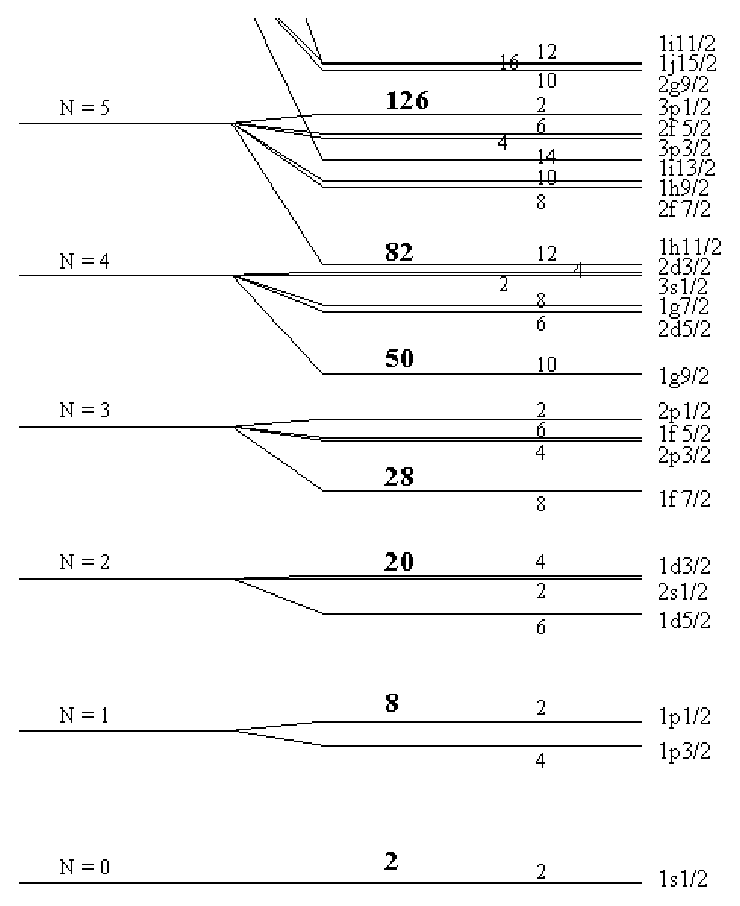
\includegraphics[width=0.5\textwidth]{shell.eps} \caption{The single-particle energy level
positions for the spherical shell model. The levels are labeled by
the quantum numbers $n\ell j$. The individual degeneracies
($2j+1$) and the cumulative degeneracies at large gaps (magic
numbers) are shown in bold faces. The lowest three major shells,
1$s$, 1$p$, 2$s$ and 1$d$, are the same as those produced by a
three dimensional, isotropic harmonic oscillator well. The higher
major shells also include the orbit with the largest $j$-values
lowered in energy from the next higher major shell by the
spin-orbit term.} \label{Fig.Shell}
\end{figure}

Apart from explaining the spin, parity, magnetic moment of the nuclei, the extended version of this model is able to explain the nuclear reaction and fusion processes as well. But this model fails to explain the large electric quadrupole moment in mid-shell nuclei which is due to large deformation of nuclear shape. The deformed nuclei are, therefore, treated separately as
discussed in the forthcoming sections. 

\subsection{Anisotropic harmonic oscillator}

\begin{figure}
\centering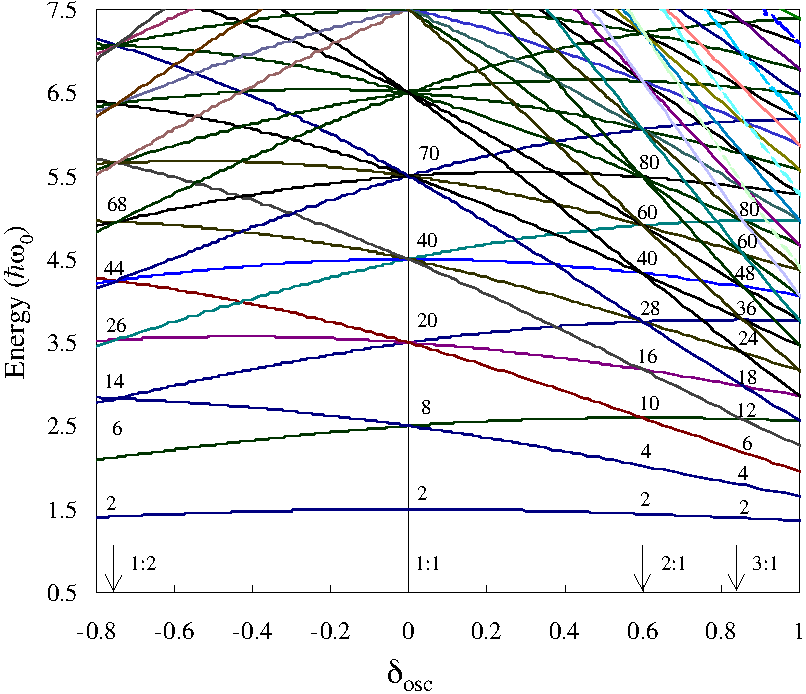
\includegraphics[width=0.7\textwidth]{aniho.png}
  \caption{\label{Fig.AniHO}Single-particle level spectrum of the
axially symmetric harmonic oscillator, as a function of
deformation($\varepsilon$). Here
$\delta_{osc}=(\omega_\rho-\omega_z)/\omega_0$  and $\omega_0
=(1/3)(2\omega_\rho+\omega_z)$. The orbit degeneracy is
$N_\rho+1$. The arrows indicate the characteristic deformation
corresponding to the ratio of $\omega_\rho/\omega_z=$ 1/2, 1/1,
2/1, and 3/1.}
\end{figure}

Anisotropic harmonic oscillator model considers the anisotropy in the potential.
Here the axial symmetry is being maintained along the $z$-axis and hence $\omega_x=\omega_y=\omega_\rho$. The Hamiltonian governing the nuclear single-particle motion becomes
\begin{equation}\label{Eq.AHOH0}
H_0 = -\frac{\hslash^2}{2m}\nabla^2  +  \frac12 m (\omega_x^2
x^2+\omega_y^2 y^2+\omega_z^2 z^2) \;.
\end{equation}
For cylindrical symmetry, the energy eigen-values corresponding to $H_0$ are given by
\begin{equation}
E_0 = (N+3/2)\hslash\omega= (n_\rho+1)\hslash\omega_\rho +
(n_z+1/2)\hslash\omega_z \;,
\end{equation}
with $N=n_x+n_y+n_z=n_\rho+n_z$.  For $\delta_{osc}=(\omega_\rho-\omega_z)/\omega_0$, the
deformation parameter in terms of the oscillator frequencies, one obtains an expression
\begin{equation}
E(n_\rho,n_z) = \hslash\omega_0 \left[
N+\frac32-\frac13\delta_{osc}(2n_z-n_\rho)\right]\;.
\end{equation}
Despite the simplicity of this model, it provides the first explanation for
the occurrence of deformation in nuclei. The appearance of shell gaps
at larger deformations leads to a situation in some nuclei such that the energy at a finite deformation is lesser than that of a spherical configuration.  
 

\subsection{Nilsson model}

In the Nilsson model, the potential in the Hamiltonian comprises the anisotropic harmonic oscillator potential plus the spin-orbit and centrifugal potentials.  The oscillator part is given by Eq.\ (\ref{Eq.AHOH0}).  Considering the case of cylindrical symmetry, and introducing a single parameter of deformation $\delta$, we can write
\begin{equation}
\omega_x^2 =  \omega_y^2 = \omega_\rho^2 = \omega_0^2[
1+(2/3)\delta] ; \ \  \omega_z^2 = \omega_0^2[ 1-(4/3)\delta ] \;,
\end{equation}
with $\omega_x \omega_y \omega_z = \omega_0^3 =$ constant, which
is the condition for the constant volume of the nucleus.  The
dependence of $\omega_0$ on $\delta$ is given by
\begin{equation}
\omega_0(\delta)= \omega^0_0 \{ [1+(2/3)\delta]^2
[1-(4/3)\delta]\}^{-1/6}=\omega^0_0 [f(\delta)] \;, \label{Eq.Cyl}
\end{equation}
where $\hslash\omega_0  =  41 A^{-1/3} [f(\delta)]$ MeV. Here we
discuss the solution in stretched coordinates defined by
\begin{equation}\label{Eq.StCoord}
    X=\sqrt{\frac{m\omega_0}{\hslash}}\ x \; ; \;\;\;
    Y=\sqrt{\frac{m\omega_0}{\hslash}}\ y \; ; \;\;\;
    Z=\sqrt{\frac{m\omega_0}{\hslash}}\ z \; .
\end{equation}
Substituting the above in Eq.\ (\ref{Eq.AHOH0}) and rearranging, one gets
\begin{equation}\label{Eq.NiH0}
    H_0=\frac12 \hslash \omega_0
    \left[-\nabla^2+r^2\right]-\delta \hslash \omega_0
    \frac43\sqrt{\frac{\pi}{5}}r^2 Y_{20} \;,
\end{equation}
where $r^2=X^2+Y^2+Z^2$ and $Y_{20}$ are the spherical harmonics. The above relation can be re-written as
\begin{equation}
    H_0=H_0^0+H_\delta \;,
\end{equation}
where the first and the second terms on the right hand side stand for the
spherical and the deformed parts respectively.  Now the total
Hamiltonian is
\begin{equation}\label{Eq.NiH}
    H=H_0^0+H_\delta+C\ \vec{l} \cdot \vec{s} + D \ \vec{l}^2 \;.
\end{equation}
The diagonal operators in this case are $\vec{l}^2,\ l_z,\
s_z$ and $j_z$ with the corresponding quantum numbers being
$l,\ \Lambda,\ \Sigma$ and $\Omega$ respectively.  With the
constraint $\Omega=\Lambda+\Sigma$, we can choose the base vector
to be $\left|N l \Lambda \Sigma \right\rangle$ and evaluate the matrix
elements.

\begin{figure}
  \centering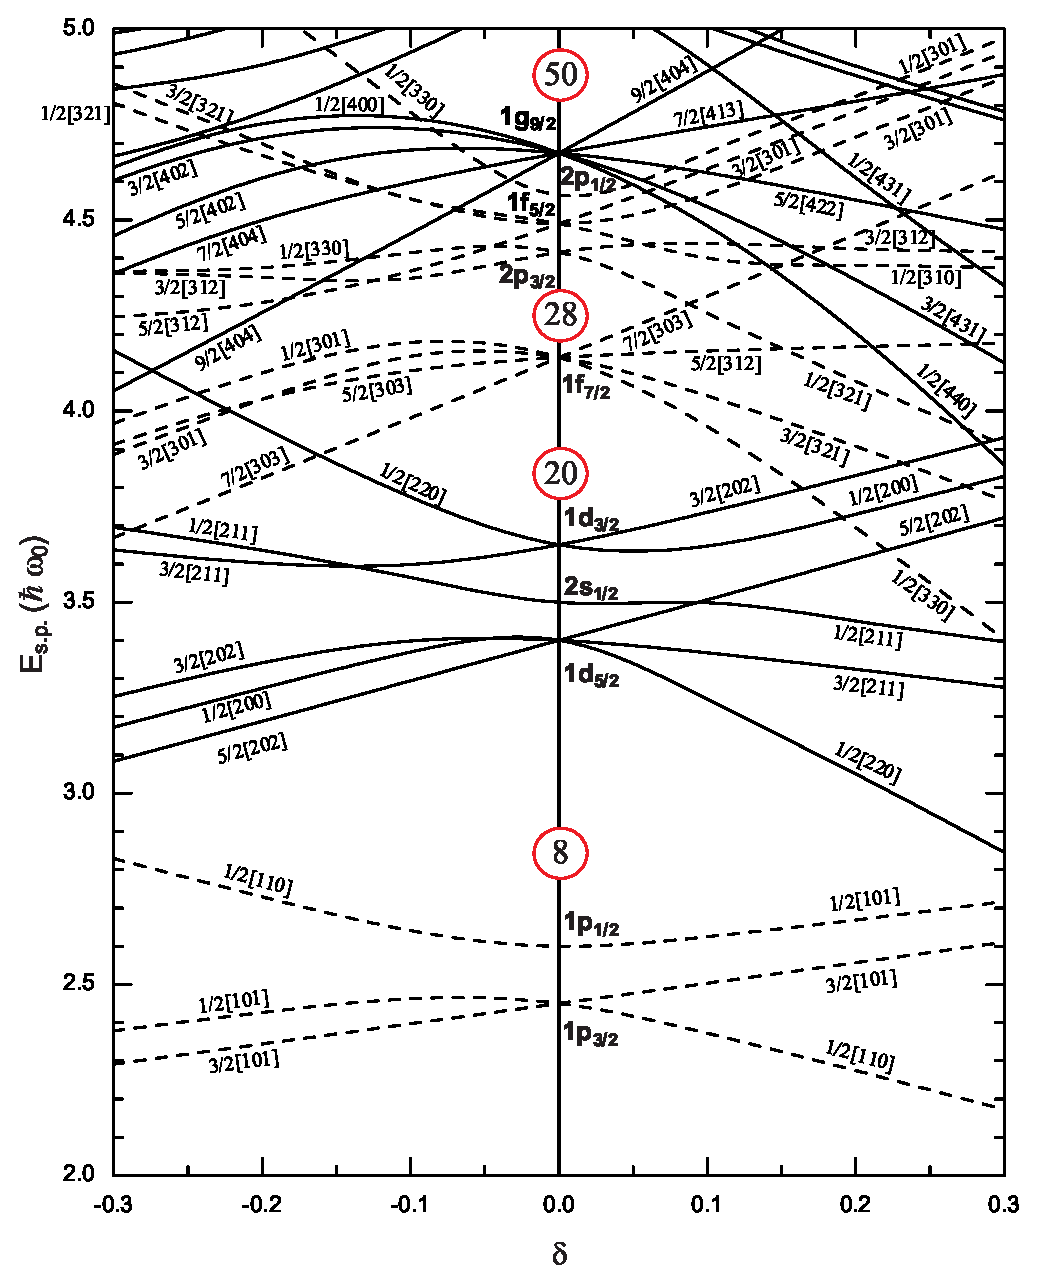
\includegraphics[width=0.9\linewidth]{nilss.eps}
  \caption{\label{Fig.NiLev} Nilsson diagram for protons and neutrons.
  Single-particle energies as a function of deformation $\delta$
  are shown for $Z$ or $N\leq 50$.  The even and odd parity levels are
  denoted by solid and dashed lines respectively.  The labeling of
  levels are by asymptotic quantum numbers $\Omega[Nn_z\Lambda]$. The value of $\kappa$ chosen is 0.05 for
  all the shells and $\mu=0.0,0.0,0.0,0.35,0.625,0.63,0.448,0.434$ for
  the first 8 shells starting from $N=0$.}
\end{figure}


Matrix elements of $H_0^0$ and $\vec{l}^2$ are diagonal and
hence,
\begin{eqnarray}
\left\langle N^\prime l^\prime \Lambda^\prime \Sigma^\prime
\right| H_0^0\left|N l \Lambda \Sigma \right\rangle &=&
\left(N+\frac32\right)\hbar\omega_0 \ \delta_{N^\prime N} \
\delta_{l^{\prime} l} \ \delta_{\Lambda^\prime \Lambda} \
\delta_{\Sigma^\prime \Sigma} \;, \\
\left\langle N^\prime l^\prime \Lambda^\prime \Sigma^\prime
\right| \vec{l}^2 \left|N l \Lambda \Sigma \right\rangle &=&
\ell (l+1) \ \delta_{N^\prime N} \ \delta_{l^{\prime} l}
\ \delta_{\Lambda^\prime \Lambda} \ \delta_{\Sigma^\prime \Sigma}
\;.
\end{eqnarray}
One can expand $\vec{l} \cdot \vec{s}$ in terms of the ladder
operators as
\begin{equation}
    \vec{l} \cdot \vec{s}
    =\frac12(\vec{l}_+\vec{s}_-+\vec{l}_-\vec{s}_+)+\vec{l}_z \vec{s}_z \,
\end{equation}
which leads to the matrix elements
\begin{eqnarray}
\nonumber \left\langle \Lambda^\prime \Sigma^\prime \right|
\vec{\ell} \cdot \vec{s} \left|\Lambda \Sigma \right\rangle &=&
\frac12 \sqrt{(\ell-\Lambda)(\ell+\Lambda+1)} \
\delta_{\Lambda^\prime \Lambda+1} \ \delta_{\Sigma^\prime
\Sigma-1} \\  \nonumber && + \ \frac12
\sqrt{(\ell+\Lambda)(\ell-\Lambda+1)} \
\delta_{\Lambda^\prime \Lambda-1} \ \delta_{\Sigma^\prime \Sigma+1} \\
&& + \ \Lambda \Sigma \ \delta_{\Lambda^\prime \Lambda} \
\delta_{\Sigma^\prime \Sigma} \;.
\end{eqnarray}
Matrix elements of $r^2$ can be calculated with the help of
recursion formulae for confluent hyper-geometric functions.
Neglecting the couplings between shells of different $N$, one
obtains
\begin{eqnarray}
\nonumber \left\langle \ell^\prime \right| r^2 \left|\ell
\right\rangle &=& \sqrt{(N-\ell+2)(N+\ell+1)} \
\delta_{\ell^\prime \ell-2} \\
\nonumber && + \ \left(N+\frac32\right) \
\delta_{\ell^\prime \ell} \\
&& + \sqrt{(N-\ell)(N+\ell+3)} \ \delta_{\ell^\prime \ell+2} \;.
\end{eqnarray}
Using the Wigner-Eckart theorem of angular momentum, one can write
the matrix elements of the spherical harmonics as
\begin{equation}
\left\langle \ell^\prime \Lambda^\prime \right| Y_{20} \left| \ell
\Lambda \right\rangle =
\sqrt{\frac{5(2\ell+1)}{4\pi(2\ell^\prime+1)}}
\left(%
\begin{array}{ccc}
  \ell & 2 & \ell^\prime \\
  \Lambda & 0 & \Lambda^\prime \\
\end{array}%
\right)
\left(%
\begin{array}{ccc}
  \ell & 2 & \ell^\prime \\
  0 & 0 & 0 \\
\end{array}%
\right) \;.
\end{equation}

With all the matrix elements available, one may set up the
Hamiltonian matrix by properly varying the quantum numbers of the
basis $\left|N \ell \Lambda \Sigma \right\rangle$. Diagonalization
of these matrices will lead to the energy eigen-values which are
the single-particle energies of nuclei within the Nilsson model. In this
model one
introduces new parameters $\kappa$ and $\mu$ instead of $C$ and
$D$.
\begin{eqnarray} \nonumber
    \kappa&=&-\frac12 \frac{C}{\hslash \omega_0^0} \;, \\
    \mu&=&\frac{2D}{C} \;.
\end{eqnarray}

The solutions of the Nilsson model, resemble those of the anisotropic oscillator with cylindrical symmetry. This also implies that at large deformation $\emph{n}_z$ becomes good quantum number. For small deformations, $j$ is an approximate quantum number, and energy of the state depends on $\Omega^{2}$. Each Nilsson state is defined by asymptotic quantum number as $\Omega[Nn_z \Lambda]$, where $n_z$ represents the number of nodes in the wavefunction along the
$z$-axis. This quantum number also signifies the spread of wavefunction along $z$-axis and hence always has greater value for low-$K$ than high-$K$ orbital, in case of prolate nuclei.

\begin{figure}[htb]
\centering
\includegraphics[width=0.9\textwidth]{nilssonEnergyN2.png}
\caption{Nilsson diagram for nucleons. Single-particle energies as a function
of deformation $\delta$ for model space $N=2$ and $\Omega=1/2$. The asymptotic quantum numbers $[Nn_z\Lambda]\Omega$ for each state are indicated on the
right side of the plot. }
\label{fig}
\end{figure}

\begin{figure}[htb]
\centering
\includegraphics[width=0.9\textwidth]{nilssonwave}
\caption{Plot of amplitudes ($|a^i_{Nlj\Omega}|^2$) for the 
Nilsson state $N=2$ and $\Omega=1/2$ in spherical basis $|Nlj\Omega\rangle$. The black
 lines show the amplitudes  for $1d_{5/2}$, red lines for $2s_{1/2}$
  and blue lines for $1d_{3/2}$ spherical components in each panel.}
\label{fig_Nil_amp}
\end{figure}

\subsubsection{Wavefunctions and admixure of $j$}

 The eigenvector ($a^i_{Nl \Lambda
 \Sigma}$) corresponding to an eigenvalue ($e_i$) enables us to obtain the wave function in Nilsson
basis such that 
\begin{equation}
\Psi_i=\sum_{Nl \Lambda \Sigma} a^i_{Nl \Lambda
 \Sigma}\left\vert N l \Lambda \Sigma \right\rangle.
\end{equation}
In spherical nuclei, $j$, the total angular momentum is a good quantum number
and hence spatial orientation of orbits is equally favored. But as the deformation is introduced, one spatial orientation is preferred over the other. Hence, there is energy dependence of the orbital orientation along the symmetry axis which can be specified by the projection of $j$ onto the symmetry axis.  This results in breakdown of the ($2j+1$) fold degeneracy. This energy drops rapidly with deformation for low $\Omega$ values and increases sharply for high $\Omega$ values. While considering full Nilsson diagram, levels with a particular $\Omega$ result from mixing of configurations with different $j$ values. For small deformation, Nilsson wavefunctions are pure in $j$ and as the deformation increases, these wavefunctions become more sensitive to configuration mixing, resulting from the non-diagonal matrix elements. For spherical nucleus this eigenvector
has only contribution from a single angular momentum $j$. For deformed
nucleus contributions from other $j$ values come into picture and this is
called $j$-mixing. As deformation increases the contribution in total wavefunction from
other $j$ values also increases.
This phenomenon of $j$-mixing can be seen explicitly if the eigenvectors
from Nilsson basis are transformed into spherical basis $\left\vert Nlj\Omega
 \right \rangle$. such that we can write 
\begin{equation}
\Psi_i=\sum_{Nl j \Omega} a^i_{Nl j \Omega}\left\vert N l j \Omega \right\rangle,
\end{equation}
where $a^i_{Nl j \Omega}$ can be understood as the mixing coefficient
of various $j$ contributing to the given Nilsson level.
This transformation
from the basis $\left\vert N l \Lambda \Sigma \right\rangle$ to $\left\vert N l j \Omega \right\rangle$ can be done using Clebsch Gordan coefficient. The relation between the coefficients $a^i_{Nl \Lambda \Sigma}$ and coefficient in spherical basis $a^i_{Nl j \Omega}$ is given by
\begin{equation}
a^i_{Nl j \Omega}=\sum_{\Lambda\Sigma}\left\langle 
l\\\ {1/2}\ \Lambda\ \Sigma|j\ \Omega \right\rangle \ a^i_{Nl \Lambda \Sigma}
\end{equation}

  The $j$-mixing can be explained using an example of a Nilsson state with $N=2$. The
state with principle quantum number $N=2$ has three orbitals  $1d_{5/2}$, $2s_{1/2}$ and $1d_{3/2}$. If the wavefunction corresponding to $\Omega=1/2$
is considered, all three $sd$ shells can mix $s$ and $d$ 
state components. Those with $\Omega=3/2$ can mix only the both 
components of $d$ shell ($1d_{5/2}$ and $1d_{3/2}$) and $\Omega=5/2$ remains
purely the $1d_{5/2}$, independent of the deformation i.e. for $\Omega=5/2$
the contribution of $1d_{5/2}$ remains unchanged with deformation. Figure (2) shows the
squared spherical component amplitudes $|a^i_{Nlj\Omega}|^2$ as a function of
deformation $\delta$ for the three $\Omega=1/2$ Nilsson states with a pure
$N=2$ space. The panels in this figure show the results for states with asymptotic
quantum numbers (a)$[220]1/2$, (b)$[200]1/2$ and (c)$[211]1/2$.  From this figure it can be clearly seen that at zero deformation the wavefunction
is purely from a single $j$ value corresponds to spherical shell. When the
 deformation increases, other $j$ components arises as
 well and the contribution from that pure $j$ state reduces.
 

\subsection{Excercises}
\begin{enumerate}
\item 
Reproduce Figs.~\ref{Fig.Shell} to \ref{fig_Nil_amp}.

\item Within Nilsson model, the energy of a nucleus with $Z$ protons and
$N$ neutrons can be obtained as
\begin{equation}
E(\delta)=\sum_{i=1}^Ze_i+\sum_{i=1}^Ne_i,
\end{equation}
where $e_i$ are the single-particle energies obtained from Nilsson model
for the given deformation $\delta$. The equilibrium shape of the nucleus
should correspond to the minimum in this energy.  One can define the deformation energy as $E(\delta)-E(\delta=0)$.  Calculate the potential energy curves
for the  Zr isotopes and verify your results with Fig.~\ref{fig_Nil_pes}.
\end{enumerate}

\begin{figure}
\center \includegraphics[width=0.7\textwidth]{pes}
\caption{Potential energy curves for Zr isotopes.}
\label{fig_Nil_pes}
\end{figure}


\section{Pairing correlations}
The nuclear structure exhibits many similarities with the electron structure
of metals.  In both cases, we are dealing with systems of fermions which may
be characterized in first approximation in terms of independent particle
motion.  Hence an analogy between the excitation spectra of nuclei and those
of the superconducting metallic state is possible.  Nuclear superfluidity is
caused by the short range attractive pairing interaction which couples
nucleons in time-reversed orbits namely in orbits with maximal spatial
overlap.  These pairs behave like bosons and condense.  The Bardeen-Cooper-%
Schrieffer \cite{BCS:1175} method of superconductivity was first applied to nuclei
by Bohr,\cite{Bohr:936} Mottelson and Pines and Belyaev, and provides accurate
description of the ground state of medium and heavy nuclei.

The pairing interaction is considered to be the most important component of
the residual nuclear interaction that couples together pairs of identical
nucleons to give total spin zero.  This interaction causes strong
configuration mixing between the available shell model states, with the
result that all the orbits of outer shell are partially filled.  This give
arise to the `quasi-particle' states and indicates the departure of nucleons
from their `independent-particle' state.

More detailed description of the theory concerned with pairing in nuclei is given elsewhere and hence not repeated.  Here
our concern is only to present an algorithmic approach to the problem and hence.

\subsection{The Ground State}
   
While applying  BCS approach in nuclear physics, the angular momentum projection on the intrinsic axis will be an important quantum number. Here we denote
the two states by $k$ and -$k$ and these  two time
reversed states are coupled by the pairing force  acting on them. The total Hamiltonian corresponding to the single-particle and the residual interaction acting on the time reversed states  is given by \cite{Greiner}
\begin{eqnarray}\label{HAM1}
\hat H=\sum_k e_{k}\ (\hat a_{k}^{\dagger}\ \hat a_{k}\ +\hat a_{-k}^{\dagger}\ \hat a_{-k})-\sum_{k\ k^{\prime}\ > 0}\langle k, -k\ |V|\ k', -k' \rangle \ \hat a_{k}^{\dagger}\ \hat a_{-k}^{\dagger}\ \hat a_{-k^{'}}\ \hat a_{k^{'}}\;.\nonumber\\
\end{eqnarray}
Here $a_k^\dagger$ and $a_k$, respectively represent the creation and annihilation operators of the state $k$ of energy $e$, and  $a_{- k}^{\dagger}$ and $a_{- k}$ those of state $-k$. For each $k>0$ state, there exist a time reversed state with $-k<0$. 
If we consider a pairing interaction with a constant matrix element, $G$ which represents the strength of the pairing interaction, we can write
\begin{equation}\label{HAM2}
\hat H=\sum_k e_{k}\ (\hat a_{k}^{\dagger}\ \hat a_{k}+\hat a_{-k}^{\dagger}\ \hat a_{- k})-G
\sum_{k\ k^{\prime}\ > 0}\hat a_{k}^{\dagger}\ \hat a_{-k}^{\dagger}\ \hat a_{-k^{'}}\
\hat a_{k^{'}}.
\end{equation}
The  analytical solution for this Hamiltonian cannot be found. In an approximate
way we can consider the Hartree mean-field approach, where the occupancy
of each state  depends on the average occupancy of the other states.  In such a case we can write the BCS state $\Psi$ as    
\begin{equation}
\label{WFN1}\Psi =\prod_{k\ >0}^{\infty}[U_k + V_k\ \hat a_{k}^{\dagger}\ \hat a_{-k}^{\dagger}]\Phi _0,
\end{equation}
where $\Phi_0$ is the vacuum state. $U_k$
and $V_k$ are the variational parameters and $U_k^2$ and $V_k^2$
give the probability of each pair of single-particle levels $(k,-k)$ is
not occupied or occupied, respectively, which has to be determined through the variational method. 
The norm of the BCS state is given by,
\begin{equation}
\label{norm}\langle\Psi|\Psi\rangle =\prod_{k\ >0}^{\infty}(U_k^2 + V_k^2),
\end{equation}
which require that $V_k^2+U_k^2=1$.
The nucleons within the pairing field are known as quasiparticles, they are connected with the original nucleons through the Bogoliubov-Valatin transformation
\cite[p.~285]{Greiner}.
The quasiparticle  is partly a particle and partly a hole \cite{Greiner}. These transformations are not commutable with the particle number operators
and the wave function resulting from this method does not represent a system
with a definite number.  Due to this reason, the BCS state is not an eigenstate of particle number operator, so the particle
number, $N_p$  is not a good quantum number for the BCS state.  However,
in the variational calculations, one can impose the constraint \begin{equation}
\label{BCS_Np}
N_{p} = \langle\Psi|\hat N|\Psi\rangle=2\sum_{k\ >0}V_k^2 \;.
\end{equation}
Since the BCS state does not obey the particle number conservation, the
desired expectation value $N_p$ can be achieved by adding the  term $\lambda
N_{p}$ to the Hamiltonian. The Lagrange multiplier $\lambda$ is fixed by the
 condition (\ref{BCS_Np}), is known as Fermi energy since it gives the increase
in energy with the change in the particle number.     The expectation value of BCS Hamiltonian $\hat H'=\hat H-\lambda
N_{p}$ can be found by minimizing the ground-state energy with respect to $V_k^2$ and yields the set of  equations
\begin{eqnarray}
\label{BCS_delta}
\Delta &=& G\sum_{k\ >0}U_kV_k\;,  \\
\label{VK2}
V_k^2&=&\frac 12\left[ 1-\frac{(e_k-\lambda )}{E_k}\right]\;,\\ 
\end{eqnarray}
where Eq.~(\ref{BCS_delta}) is known as the gap equation. The quantity $\Delta$ is known as the pairing gap. $E_k$ is the quasiparticle energy, $E_k=\sqrt{(e_k-\lambda )^2+\Delta^2}$. Effectively, the  pairing interaction smoothens the level occupancy near the Fermi level over the range $\Delta$. 

The BCS equations (\ref{BCS_Np}) and (\ref{BCS_delta}) can be rewritten
as
\begin{eqnarray}
\label{BCS1}
N_p & = & \sum_{k =1}^{N_p}{\left\{1-\frac{e_k-\lambda}
{\left[(e_k-\lambda)^2+\Delta^2\right]^{1/2}}\right\}}\;, \quad \text{and}\\
\label{BCS2}
\frac 2G & = &\sum_{k=1}^{N_p}{\left\{\frac{1}
{\left[(e_k-\lambda)^2+\Delta^2\right]^{1/2}}\right \}}.
\end{eqnarray}
Pairing can be dealt with either the constant gap ($\Delta$) approximation or the constant strength ($G$) approximation. In the former approach, $\Delta$ is chosen to be a constant value usually estimated from the odd-even mass differences \cite[p.~170]{bohr1} or taken as the average empirical value $12/\sqrt{A}$ MeV. In such a case only Eq.~(\ref{BCS1}) has to be solved to obtain $\lambda$. In the latter approach, for a given value of $G$, both the Eqs.~(\ref{BCS1}) and (\ref{BCS2}) have to be solved simultaneously to obtain $\Delta$ and $\lambda$ using the Newton's method as described in appendix-\ref{newtonsmethod}.

\subsection{Solving the BCS equations}
\label{SBCS}
The pairing energy necessarily depends on the following quantities.
\begin{enumerate}
\item The single-particle energy levels ($e_k$).
\item the constants
\subitem $G_{p,n}$ -- pairing force strength parameters (for protons and neutrons respectively).
\subitem $N_p$ -- number of single-particle states included in the pairing window.
\item the variables
\subitem $\Delta$ -- the pairing gap.
\subitem $\lambda$ -- the level of surface of the Fermi sea.
\end{enumerate}

The pairing energy is calculated using the following algorithm.
\begin{enumerate}
\item The single-particle energy levels ($e_k$) obtained form the
diagonalization of the modified oscillator (MO) Hamiltonian 
are used.  Here the suffix $k$ stands for single-particle levels which are
doubly degenerate.  Hence in the corresponding single-particle energy matrix,
only the odd elments are considered for constructing $e_k$.

\item For the modified oscillator potential a typical choice could be
\begin{equation}
G_{Z,N} = [19.2\pm7.4(N-Z)]/A^2 \text{ MeV}.
\end{equation}
In these calculations $\sqrt{15} Z$ and $\sqrt{15} N$ single-particle states above and below the Fermi level are included.

\item $N_p$ is equal to $Z \ (N)$ for protons (neutrons) counting from the
bottom of the well.  However the count is reduced by
unity in the case of odd $Z$ (or $N$) to make $N_p$ even.

\item The values $\Delta$ and $\lambda$ are determined by solving the set of
equations
\begin{eqnarray}
\label{BCS1}
N_p & = & \sum_{k=1}^{N_p}{\left\{1-\frac{e_k-\lambda}
{\left[(e_k-\lambda)^2+\Delta^2\right]^{1/2}}\right\}} \\
\label{BCS2}
\frac 2G & = & \sum_{k=1}^{N_p}{\ \ \ \frac{1}
{\left[(e_k-\lambda)^2+\Delta^2\right]^{1/2}}}
\end{eqnarray}

These equations are solved using the Newton's method.

\item The occupation probabilites ($v_k^2$) are calculated using the relation
\begin{equation}
\label{vk2}
v_k^2  = \frac 12 \left\{1-\frac{e_k-\lambda}
{\left[(e_k-\lambda)^2+\Delta^2\right]^{1/2}}\right\} \ \ \ k=1,2,...N_p
\end{equation}

\item Finally the Pairing energy is calculated using the relation
\begin{equation}
E_{PC} = 2 \left( \sum_{k=1}^{N_p}{e_k \ v_k^2} -
    \sum_{k=1}^{\frac 12 N_p}{e_k} \right) - \frac{\Delta^2}{G}
    -G \left( \sum_{k=1}^{N_p}{v_k^4} -
    \sum_{k=1}^{\frac 12 N_p}{1} \right)
\end{equation}
\end{enumerate}

\section{Hot nuclei}
\subsection{Useful relations}
The effect of temperature ($T$) comes in picture through the single-particle occupation number, which can
be expressed in terms of Fermi-Dirac distribution, and  is given by 
\begin{equation}\label{NIT}
n_i=\frac 1{1+\exp \left( \frac{e_i-\lambda }T\right)}\;,
\end{equation}
where $\lambda$ is the chemical potential which guarantees the particle number conservation through the constraint
\begin{equation}
N_p=\sum_{i}^\infty n_i,
\end{equation}
 where $N_p$
is the total number of particles. It is useful to have the derivative of
the occupation numbers which should mean the single-particle level density
and is given by
\begin{equation}\label{GTEMP}
g(e)=\sum_{i=1}^\infty \left.
\frac{dn_i(e_i,\lambda )}{ d\lambda }\right| _{\lambda
=e}=\sum_{i=1}^\infty\frac 1{4T\cosh ^2[(e-e_i)/2T]}.
\end{equation}
The single-particle entropy is given by
\begin{equation}
s_i=-\left[ n_i\ln n_i+\left( 1-n_i\right) \ln \left(
1-n_i\right) \right],
\end{equation}
and hence the total entropy of the system 
\begin{equation}
S=\sum_i^\infty s_i.
\end{equation}
The free energy is given by
\begin{equation}\label{F}
F=E^T-TS,
\end{equation}
where the internal energy $E^T$ is given by 
\begin{equation}
E^T=\sum_{i=1}^{N_p} e_in_i.
\end{equation}

\section{Quantum Hadrodynamics} 

Physical systems that involve an infinite number of degrees of freedom can conveniently be described by some sort of field theory. Almost all systems in nature involve an extremely large number of degrees of freedom. For instance, a droplet of water contains of the order of $10^{26}$ molecules and while each water molecule can in many applications be described as a point particle, each molecule has itself a complicated structure which reveals itself at molecular length scales. To deal with this large number of degrees of freedom, which for all practical purposes is infinite, one often regards a system as continuous, in spite of the fact that, at small enough distance scales, it is discrete. This system is not described by specifying the equations of motion for each molecule separately, but instead the displacement field is used as the dynamical variable, which, being continuous, comprises an infinite number of degrees of freedom. In classical mechanics, field theory is thus obviously important for continuous systems. But also, electromagnetic phenomena are described on the basis of a field theory. In Maxwell�'s theory of electromagnetism, the basic dynamical variables are the electric and magnetic fields. In terms of these fields one can both understand the electromagnetic forces between charges and the phenomenon of electromagnetic radiation. The methods of classical mechanics can be suitably formulated so that they can be used for continuous systems. However, to give a quantum-mechanical treatment of field theory is much more difficult and requires new concepts. Thus, quantum field theory (QFT) provides a theoretical framework for constructing quantum mechanical models of systems classically parametrized (represented) by an infinite number of dynamical degrees of freedom, that is, fields and many-body systems. 

In perturbative quantum field theory, the forces between particles are mediated by other particles. That is in a mathematical language, any model in perturbative QFT, for eg: here the $\sigma-\omega$ model, can explain the nuclear matter by the interaction of nucleons and $\sigma$ and $\omega$  mesons. So, such a model can be described by a Lagrangian which contains all the particles in the model and their mutual interactions. Now in QFT, each particle is represented by a field which is defined over the $4$-dimensional space-time. The interactions among the particles are represented by terms which show the coupling of different kinds of fields at the same space-time point.


Now, before we proceed to understand the interactions of nuclear matter,
let us try to understand this from a simple model of quantum electrodynamics, which is the quantum field theory of electromagnetic force. The quantum field theory approach visualizes the force between the electrons as an exchange force arising from the exchange of virtual photons. It is represented by a series of Feynman diagrams, the most basic of which is shown in the Fig.~\ref{fig:qed}
\begin{figure}\begin{center}\includegraphics[width=0.3\textwidth]{qed.png}\end{center}\vspace{-34pt}
\caption{Feynman digaram of electron-positron interaction.}\label{fig:qed}
\end{figure}
In this figure the solid line shows the particles and the wavy line represents
the virtual particle, here, it is, the photon. Then, by techniques available one can write the Lagrangian for this system.
The Lagrangian for the QED system is given as,
\begin{equation}
\mathcal{L}=-\frac{1}{4}F_{\mu \nu}F^{\mu \nu}+\bar\psi(i\gamma^{\mu}\partial_{\mu}-m)\psi-e\bar\psi\gamma^\mu
\psi A_\mu \label{eq:qed}
\end{equation} 
where $\psi$, $\bar\psi$ and $A_{\mu\nu}$ represent fields of electron,
positron and photon, respectively and $F_{\mu\nu}$ is the electromagnetic
field strength and  \begin{equation}
F_{\mu \nu}=\partial_\mu A_\nu-\partial_\nu A_\mu \;.
\end{equation}
The first term in Eq.~(\ref{eq:qed}) represents the non-interacting dynamics of the photon field
and second term represents the non-interacting dynamics of the fields of electron and positron. The third term couples all the three fields and hence describes their interaction, for eg: annihilation of an electron and positron pair into a photon.


Applying this same approach on to the nuclear system, we have the QHD. In the formalism of QHD, baryons and mesons are the degrees of freedom and we say the nucleons interact through the exchange of virtual mesons by which the effects of relativistic propagation are naturally incorporated.  Here we discuss the simplest version in which we will study the nuclear matter using the linear $\sigma-\omega$ model (QHD-I).

$\sigma$  is a neutral scalar meson with spin parity, $J^{p}=0^{+}$. and has mass of about, $m_{s}=500$ MeV/c$^{2}$. $\omega$ is neutral vector meson with  spin parity,  $J ^{p}=1^{-}$ and has mass of about, $m_{v}=782$ MeV/$c^{2}$. Thus, only vector field, $V_{\mu}$ (of omega mesons) and a scalar field, $\phi$ (of sigma mesons) are needed to describe the nuclear interaction. Thus, the nuclear potential curve is accounted by the $\sigma-\omega$ mesons,where the hard core repulsive part of the potential is accounted by the $\omega$-mesons and the attractive part is accounted by the $\sigma$-mesons (Fig.~\ref{QHD_potential}). The baryons are described by the field, $\psi$. 

\begin{figure}[h]\begin{center}\includegraphics[width=0.98\textwidth]{QHDpotential.png}\end{center}\vspace{-28pt}
\caption{Inter-nucleon potential in terms of the potentials of $\sigma$ and
$\omega$ mesons.}
\label{QHD_potential}
\end{figure}

Correspondingly, the Lagrangian density for the system is:
\begin{equation}
L=\bar\psi[ \gamma_{\mu}(i\partial^{\mu}-g_{\nu}V^{\mu})-(M-g_{s}\phi)]\psi+
\frac{1}{2}(\partial_{\mu}\phi\partial^{\mu}\phi-m^{2}_{s}\phi^{2})-\frac{1}{4}F_{\mu\nu}F^{\mu\nu}+\frac{1}{2}m^{2}_{\nu}V_{\mu}V^{\mu}, \label{Lagrangian density}
\end{equation}
where $F_{\mu\nu}=\partial_{\mu }V_{\nu}-\partial_{\nu}V_{\mu}\;,$ and
$-\frac{1}{4}F_{\mu\nu}F^{\mu\nu}+\frac{1}{2}m^{2}_{\nu}V_{\mu}V^{\mu}$ represent the non-interacting dynamics of $\omega$-meson field,
$\frac{1}{2}(\partial_{\mu}\phi\partial^{\mu}\phi-m^{2}_{s}\phi^{2})$ represents the non-interacting dynamics of $\sigma$-meson field.
$\bar\psi[ \gamma_{\mu}(i\partial^{\mu}-g_{\nu}V^{\mu})-(M-g_{s}\phi)]\psi
$ represents

a) non-interaction dynamics of baryon field,

b) interaction of the baryons and $\omega$-meson,

c) interaction of the baryons and $\sigma$-meson,

\noindent and $M-g_{s}\phi$ represents the effective mass of the baryons.

Now we use the Euler Lagrange equation
\begin{equation}
\frac{\partial}{\partial x^{\mu}}\left[\frac{\partial L }{\partial(\partial q_{i}/\partial x^{\mu})}\right]-\frac{\partial L}{\partial q_{i}}=0
\end{equation}
as a constraint to derive field equations using this Lagrangian density, which gives us three field equations:
\begin{equation} 
(\partial_{\mu}\partial^{\mu}+m^{2}_{s})\phi=g_{s}\bar\psi\psi,
\end{equation}
\begin{equation}
\partial_{\mu }F^{\mu\nu}+m^{2}_{\nu}V^{\nu}=g_{\nu}\bar\psi\gamma^{\mu}\psi,
\end{equation}
\begin{equation}
[\gamma^{\mu}(i\partial_{\mu}-g_{\nu}V_{\mu})-(M-g_{s}\phi)]\psi=0.
\end{equation}
Next the energy momentum tensor is given by 
\begin{equation}
T_{\mu\nu}=-g_{\mu\nu}L+\frac{\partial q_{i} }{\partial x^{\nu}}\frac{\partial
L}{\partial (\partial q_{i}/\partial x_{\mu})},
\end{equation}
where $g_{\mu\nu}$ is the Lorentz transformation matrix given by $\begin{pmatrix}1 & 0 & 0 & 0\\ 0 & -1 & 0 & 0 \\
0 & 0 & -1 & 0 \\
0 & 0 & 0 & -1 \\
\end{pmatrix}$and $\mu$, $\nu=0,1,2,3.$

The first diagonal element of the energy-momentum tensor, $T_{00}$ gives
the energy density and the mean value of the remaining diagonal elements
gives the pressure. That is, Energy density, $\mathcal{E}= T_{00 }$, Pressure, $P=\frac{1}{3}\left\langle T_{ii}\right\rangle$.

Considering uniform nuclear matter, the ground state of the system is obtained
by filling states with wave number \(\textbf{k}\) and spin-isospin degeneracy
$\gamma=4$ for nuclear matter (neutrons and protons with spin up and down)
and $\gamma=2$ for neutron matter (only neutrons with spin up and down).
Finally, we get the expressions,
\begin{equation}  
\mathcal{E}=\frac{g^{2}_{\nu}}{2m^{2}_{\nu}}\rho^{2}_{B}+\frac{m^{2}_{s}}{2g^{2}_{s}}(M-M^{*})^{2}+\frac{\gamma}{(2\pi)^{3}}\int^{k_{F}}_{0}d^{3}k(k^{2}+M^{*2})^{1/2},
\label{EQ_energy}
\end{equation}
\begin{equation}
P=\frac{g^{2}_{\nu}}{2m^{2}_{\nu}}\rho^{2}_{B}-\frac{m^{2}_{s}}{2g^{2}_{s}}(M-M^{*})^{2}+\frac{1}{3}\frac{\gamma}{(2\pi)^{3}}\int^{k_{F}}_{0}d^{3}k\frac{k^{2}}{(k^{2}+M^{*2})^{1/2}}.
\label{EQ_pressure}
\end{equation}
Thus, we get the expressions for energy and  pressure in terms of baryon density, $\rho_{B}$ as Fermi wave vector, $k_{F}$ and baryon density, $\rho_{B}$ are related to each other by the relationship,
\begin{equation}
\rho_{B}=\frac{\gamma}{(2\pi)^{3}}\int^{k_{F}}_{0}d^{3}k=\frac{\gamma}{6\pi^{2}}k^{3}_{F}.
\end{equation}
The first two terms in the Eq.~(\ref{EQ_energy}) and Eq.~(\ref{EQ_pressure}) arise from the mass terms for the vector and scalar fields. The final terms in these equations are those of a relativistic Fermi gas of baryons of mass $M^{*}$. These expressions give the equation of state of nuclear matter in parametric form: $\mathcal{E}$($\rho_{B}$) and $P(\rho_{B})$.


Now, it remains to determine the effective mass $M^{*}$, to completely
determine the energy density and pressure in terms of baryon density, $\rho_{B}$. This is done by minimizing $\mathcal{E}(M^{*})$ with respect to $M^{*}$ leading to the self -consistency relation 
\begin{equation}
M^{*}=M-\frac{g^{2}_{s}}{m^{2}_{s}}\frac{\gamma}{(2\pi)^{3}}\int^{k_{F}}_{0}d^{3}k\frac{M^{*}}{(k^{2}+M^{*2})^{1/2}}.
\end{equation}
This then yields the transcendental self-consistency equation for the effective
mass:
\begin{equation}
M^{*}=M-\frac{g^{2}_{s}}{m^{2}_{s}}\frac{\gamma M^{*}}{4\pi^{2}}\left[ k_{F}E^{*}_{F}-M^{*2}\ln\left(\frac{k_{F}+E^{*}_{F}}{M^{*}}\right)\right],
\label{Eq_effective_mass}
\end{equation}
where $E^{*}_{F}=(k^{2}_{F}+M^{*2})^{1/2}.$
\\Now, solving the transcendental equation of effective mass ($M^{*}$) Eq.~(\ref{Eq_effective_mass}), numerically, we get the curves shown in the Fig.~\ref{effective mass}, for neutron matter ($\gamma=2$) and nuclear matter ($\gamma=4$).

\begin{figure}[h]\begin{center}\includegraphics[width=0.98\textwidth]{effectivemass.png}\end{center}\vspace{-28pt}
\caption{Effective mass as a function of Fermi momentum ($k_F$) for nuclear matter ($\gamma=4$)
and
neutron matter ($\gamma=2$), within QHD-1.}
\label{effective mass}
\end{figure}

We can see that as baryon density, $\rho_{B}$,  increases the effective mass
decreases. We know that $M^{*}=M-g_{s}\phi$, where $\phi$ corresponds
to the field of scalar $\sigma$ mesons which account for the attractive strong
force. So, when the density increases the nucleons come closer to each other
that is one comes in the immediate influence of each others strong attractive
nuclear force. Thus, the field, $\phi$, becomes dominant and so the factor
$g_{s}\phi$ increases and thereby, the effective mass, $M^{*}$, decreases.


Also, we have plotted the binding energy per nucleon, $\frac{E}{\rho_{B}}-M$, against the Fermi wave-vector, $k_{F}$ (Fig.~\ref{BE}).

\begin{figure}[h]
\begin{center}
\includegraphics[width=0.98\textwidth]{bindingenergy.png}
\end{center}
\vspace{-28pt}
\caption{Saturation curve for symmetric and neutron matter
within QHD-1.}
\label{BE}
\end{figure}

As a next step, solving for the pressure we get the curves as shown in Fig.~\ref{pressure}.

\begin{figure}[h]
\begin{center}
\includegraphics[width=0.98\textwidth]{pressure.png}
\end{center}\vspace{-28pt}
\caption{Pressure, $P$, against Fermi momentum ($k_F$) for symmetric matter
and neutron matter within QHD-1.}
\label{pressure}
\end{figure}

\section{Nuclear chart}
Following the periodic table for atomic elements, nuclear physicists have plotted all the nuclide in a methodical way as shown in the nuclear chart Fig.~\ref{nuclchart}. The nuclide are placed in the chart according to their number of protons and neutrons, where $x$-axis represents the number of neutrons $N$, and  $y$-axis the number of protons, $Z$. 
The stable nuclides, labeled in the chart as naturally abundant, define a region called the stability valley. For lower masses ($A=Z+N$), $N=Z$ corresponds
to the stability line and for higher masses, this line corresponds to $N>Z$
which can be explained by a simple liquid drop model considering Coulomb
and asymmetry effects. Above the stability line one has a neutron deficient region where there are too few neutrons in the nuclei, for them to be stable against radioactive decay. As one goes on adding protons to a nucleus in the stability valley, one will land in the region where the Coulomb repulsion becomes so large that the strong nuclear forces are not able to hold the nuclei in its bound state. The extra proton added drips out of the nucleus, as its proton separation energy ($S_p$) becomes zero. This limit is known as the `\textit{proton drip line}'.   Similarly, as we keep on adding neutrons
to a particular nucleus in the stability valley, we reach the `\textit{neutron drip line}' and along the neutron drip line the neutron separation energy
($S_n$) for a single neutron is zero. According to the traditional nuclear physics point of view, no bound nuclei can be found beyond these lines. So far, most of the proton drip line nuclei have been produced but a large number of neutron drip line nuclei are yet to be discovered. This region is known as `\textit{Terra Incognita}' or the unknown territory.

\begin{figure}\center
\includegraphics[width=1.2\textwidth]{nuclchart.png}
\caption{The chart of nuclides.  Every point here represents a specific
combination of neutrons and protons and hence a particular nucleus. The colors
depict the stability as given in the legend. \label{nuclchart}}
\end{figure}
 

\subsection{The semi-empirical mass formula}

We can express the mass of a nucleus ($M(N,A)$) as a function of $N$ and $Z$ as
\begin {equation}\label{masseq}
M(N,A)c^{2}=NM_{n}c^{2}+ZM_{H}c^{2}-B(N,Z),
\end {equation}
where $M_n$ is the mass of a neutron, $M_H$ is the mass of the proton and $B$ is the binding energy of the nucleus.  Using the semi-empirical mass formula, the above Eq.(\ref{masseq}) can be written as 
\begin {equation}
M(N,A)c^{2}=N(M_{n}-M_{H})c^{2}+AM_{H}c^{2}-a_{v}A+a_{s}A^{2/3}+a_{c}\frac{Z^{2}}{A^{1/3}}+a_{sym}\frac{(N-Z)^2}{2A},
\end {equation}
where the constants are fitted to reproduce the experimentally measured binding
energies as $a_v=-16$ MeV, $a_s=20$ MeV, $a_c=0.751$ MeV, $a_{sym}=21.4$ MeV. For maximum stability ($\beta$-stability), we have the condition $\frac{\partial M}{\partial N}=0$ which yields the relation
\begin{equation}\label{betastability}
N-Z=\frac{a_{c}A^{2/3}-(M_n-M_H)c^2}{2a_{sym}/A+a_{c}/A^{1/3}}.
\end {equation}



\subsection{Proton drip line}
The proton drip line is characterized by the condition $\frac{\partial B(N,Z)}{\partial Z}=0$. Employing the semi-empirical mass formula, we get 
\begin{eqnarray}
\frac{\partial B(N,Z)}{\partial Z}&=&a_v-\frac{2}{3}a_s(N+Z)^{-1/3}-\frac{2a_cZ}{(N+Z)^{1/3}}+\frac{a_c}{3}\frac{Z^2}{(N+Z)^{4/3}}\nonumber\\
&&+a_{sym}\frac{(N-Z)}{(N+Z)}+a_{sym}\frac{(N-Z)^2}{2(N+Z)^2}.
\end{eqnarray}
Substituting $N+Z=A$ and $N=A-Z$, leads to the relation
\begin{equation}
Z^2 \left( \frac{a_c}{3A^{4/3}}+\frac{2a_{sym}}{A^2} \right)-Z \left( \frac{2a_cA}{A^{4/3}}+\frac{4a_{sym}A}{A^2} \right)+a_v-\frac{2}{3}a_s\frac{1}{A^{1/3}}+\frac{3}{2}a_{sym}=0\ .
\end{equation}
The above equation has the form
\begin{equation}
Z^2-2ZA(1+\beta) +\gamma A ^2=0,
\end{equation}
from which we obtain 
\begin{equation}\label{protondrip}
Z= A\left\{(1+\beta)\pm\sqrt{[(1+\beta)^2-\gamma]}\right\},
\end {equation}
where 
\begin{equation}
\beta=\frac{2a_cA^{2/3}}{a_cA^{2/3}+6a_{sym}}, \quad
\gamma=\frac{a_v +\frac{3}2a_{sym}-\frac{2}{3}a_sA^{-1/3}}{\frac{1}{3}a_cA^{2/3}+2a_{sym}}.
\end{equation}

\subsection{Neutron  drip line}
The neutron drip line is characterized by the condition $\frac{\partial B(N,Z)}{\partial N}=0$. With the binding energy expressed as a function of $N$ and $Z$, the partial derivative can be obtained as 
\begin {equation}
\frac{\partial B(N,Z)}{\partial N}=a_v-\frac{2}{3}a_s(N+Z)^{-1/3}+\frac{a_c}{3}\frac{Z^2}{(N+Z)^{4/3}}-a_{sym}\frac{(N-Z)}{(N+Z)}+a_{sym}\frac{(N-Z)^2}{2(N+Z)^2}.
\end {equation}
Substituting $N+Z=A$ and $Z=A-N$, leads to the equation,
\begin {equation}
N^2 \left(\frac{a_c}{3A^{4/3}}+\frac{2a_{sym}}{A^2}\right)-N\left(\frac{2a_cA}{3A^{4/3}}+\frac{4a_{sym}A}{A^2} \right)+a_v-\frac{2}{3}a_s\frac{1}{A^{1/3}}+\frac{a_c}{3}A^{2/3}+\frac{3}{2}a_{sym}=0\ .
\end{equation}
This equation has the form
\begin{equation}
N^2-2NA +\alpha A^2=0,
\end{equation}so that
\begin{equation}\label{neutrondrip}
N=A\left[1\pm\sqrt{(1-\alpha)}\right],
\end{equation}
where
\begin{equation}
\alpha=\frac{a_{v}+\frac{3}{2}a_{sym}-\frac{2}{3}\frac{a_s}{A^{1/3}}+
\frac{a_c}{3}A^{2/3}}{\frac{a_c}{3}A^{2/3}+2a_{sym}}.
\end{equation}
With the constants inserted, we get the nuclear landscape having the $\beta$-stability
line [Eq.~(\ref{betastability})], the proton drip line [Eq.~(\ref{protondrip})] and the neutron drip line [Eq.~(\ref{neutrondrip})]  as depicted in Fig.\ \ref{Drip_line}.
\begin{figure}
\center
\includegraphics[width=0.82\textwidth]{driplines.pdf}
\caption{Nuclear chart comprising the $\beta$-stability
line [Eq.~(\ref{betastability})], the proton drip line [Eq.~(\ref{protondrip})] and the neutron
drip line [Eq.~(\ref{neutrondrip})]  , calculated using a
simple semi-empirical
mass formula.}\label{Drip_line}
\end{figure}

\begin{figure}
\center
\includegraphics[width=0.99\textwidth]{wells.png}
\caption{\label{Fermilevels}Schematic representation of Fermi levels for $\beta$-stable, proton drip line and neutron drip line nuclei. No $\beta$-decay is possible in $\beta$-stable
nuclei.}
\end{figure}

\begin{figure}
\center
\includegraphics[width=1.0\textwidth]{nuclidetrail.png}
\caption{Number of isotopes discovered in every year until the year 2010 (After Ref.~\cite{Thoennessen:25}).  In the years 2011 and 2012, the number
of new nuclei identified are 7 and 67, respectively \cite{Thoennessen:056301}.
New discoveries have been
closely linked to new technical developments of accelerators
and detectors.}\label{nucleartrail}
\end{figure} 

\subsection{Experimental scenario}
The experimental search for mapping the drip lines has gathered momentum
in the last few decades thanks to the development of new techniques and facilities.
 The time evolution with the color codes representing the year of publication (recognized discovery) was presented in Fig~\ref{nuclchart}. A more recent compilation \cite{Thoennessen:25} of the discovery of isotopes is presented in Fig.~\ref{nucleartrail}, where one can notice that more than
100 isotopes were discovered in the year 2010. In the year 2011, only
seven new isotopes were discovered. The pace of discovery picked up again
in the year 2012 with the identification of 67 new nuclei,  leading to a total of 3105 nuclides observed by the end of 2012 \cite{Thoennessen:056301}. The 3015 nuclides currently reported in the published literature still probably constitute less than 50\% of all nuclides that potentially could be observed. Thus the quest for the discovery of nuclides that were never made on Earth continues to be a strong motivation to advance nuclear science toward the understanding of nuclear forces and interactions. The discovery of a nuclide is the first necessary step to explore its properties.

All the nuclei waiting to be discovered are quite unstable and  radioactive.
 The study of these radioactive nuclei presents a great challenge, since they are involved in the paths for nucleosynthesis processes, that lead to the creation of matter in the universe \cite{Erler:509}. At the same time they are needed for tests of symmetries, important to establish the Standard Model of fundamental interactions. On the neutron rich side it is even impossible to predict the limits of stability, known experimentally only up to fluorine, since models strongly depend on parameters that are not precisely determined from the properties of stable nuclei. Nuclear models that describe stable nuclei, may not be adequate for this region, which is of great importance to understand the various astrophysical scenarios for rapid neutron capture processes.




\section{Alpha Decay}
The nuclei far from the $\beta$-stability valley are generally unstable and  decay through many decay processes,  e.g. p, n, $\beta$, $\gamma$, $\beta+$ cluster, Electron Capture (EC) etc. These unstable nuclei undergo nuclear decay to become more stable. Here we discuss the $\alpha$-decay process, which is a type of cluster-decay. $\alpha$-decay is the radioactive emission of $\ ^{4}_{2}He\ $ nucleus, consisting two protons and two neutrons. Two is the magic number for both proton and neutron, so $\alpha$-particle is more stable than neighbouring nuclei, and in $\alpha$-decay process the daughter nucleus has four nucleons fewer than the parent nucleus.
\begin{equation}
_{(Z+2)}^{(A+4)}P=_{Z}^{A}D+\alpha\ .
\end{equation}
 The $Q_\alpha$-value of the decay is the difference of the mass of the parent and the combined mass of the daughter and the $\alpha$-particles.
 \begin{equation}
 Q_\alpha=(m_P-m_D-m_\alpha)c^2\ .
 \end{equation}
 The mass difference between the parent and daughter nucleus can easily be estimated by Liquid Drop Model. It is also equal to the difference between the sum of the binding energies of the daughter and the $\alpha$-particles and that of the parent nucleus.
 
 The lifetime of $\alpha$-decay varies from the order of $10^{-7}$ seconds to $10^{10}$ years. $\alpha$-particle inside the nucleus is in quasi-bound-state. It is bound to an attractive potential well created by the strong, short-range, nuclear force and also there is a Coulomb repulsion between the quasi-$\alpha$-particle and rest of the nucleus. Thus these two competing forces balance in such a way that it creates a barrier for $\alpha$-particle ($^{4}_{2}He$-nucleus). The nucleus has a small probability of escaping outside using quantum mechanical tunneling effect. This tunneling probability depends on the height and width of the wall or barrier and related to the transmission coefficient $T$. 
Here we discuss the WKB method with different potentials for calculating half-life of $\alpha$-decay.
 \subsection{Square-well plus Coulomb potential}
 Here we consider the nuclear potential as a square-well potential and after the nuclear surface (the nuclear radius $R$) the potential is Coulomb potential
given by \begin{equation}
V(r)=\begin{cases}-V_{0}& \text{for } r\leqslant R \\
 \frac{2Ze^2}{4\pi\epsilon_0r} & \text{for } r>R \end{cases}
\end{equation}
where \(V_0\)\(=50\) MeV is the depth of the potential well.\\
In graphical representation of above potential,
\begin{figure}[ht!]
\centering
%\resizebox{15cm}{!}
\includegraphics[width=0.7\textwidth]{SquarewellCou.png}
\caption{Finite range square-well potential and outside $R$ the potential is coulomb potential for $\alpha$-decay from $^{212}\text{Po}$.}
\label{squarewell}
\end{figure}
height of the potential barrier is V and width is $\Delta r=b-R$. Suppose we have a wave packet representing $\alpha$-particle with mass $m_\alpha$ and kinetic energy $E$. Then the transmission coefficient is given by\\
\begin{equation}
T\approx \text{e}^{-2k\Delta r}
\end{equation}
where
\begin{equation}
k=\sqrt{2m_\alpha\left\vert V-E \right\vert}/\hslash\ . \label{eq:kalpha}
\end{equation}
This can be extended to any barrier shape in the form of the WKB approximation.
\begin{equation}
T\approx \text{exp}\left(-2\int_R^b k(r)dr\right)=\text{exp}(-2G)\ . \label{eq:trcoeff}
\end{equation}
In general $R$ and $b$ are the classical turning points of the motion inside and outside the barrier. Here in Fig (1), $R$ is the radius of the nuclear potential.\\
We can approximately equate the energy release ($Q$) in the $\alpha$-decay to the kinetic energy ($E$) of the $\alpha$-particle and to the potential at the outer classical turning point ($b$).
\begin{equation}
Q\approx E=\frac{Z_\alpha Z_De^2}{4\pi\epsilon_0b}\ ,
\end{equation}
or
\begin{equation}
b=\frac{Z_\alpha Z_De^2}{4\pi\epsilon_0Q}\ .
\end{equation}
Plugging Eqs.~(\ref{eq:kalpha}) and (125) in Eq.~(\ref{eq:trcoeff}), then the integral over $k(r)$ becomes
\begin{eqnarray}
&&2G=\frac{2}{\hslash}\sqrt{2m_\alpha Q}
\int_R^b\left[\frac{b}{r}-1\right]^{1/2}dr\ ,\\
\Rightarrow\quad&&2G=\frac{2b}{\hslash}\sqrt{2m_\alpha Q}
\left[\text{cos}^{-1}\left(\frac{R}{b}\right)^{1/2}-
\left(\frac{R}{b}\right)^{1/2}\left(1-\frac{R}{b}\right)^{1/2}\right]\ ,\\
\Rightarrow\quad&&2G=\frac{2Z_\alpha Z_D e^2}{4\pi\epsilon_{0}}
\sqrt\frac{2m_\alpha}{\hslash^2 Q}
\left[\text{cos}^{-1}\left(\frac{R}{b}\right)^{1/2}-
\left(\frac{R}{b}\right)^{1/2}\left(1-\frac{R}{b}\right)^{1/2}\right]\ .
\end{eqnarray}
Where the kinetic energy of $\alpha$-particle is
\begin{equation}
Q=\frac{1}{2}m_\alpha v^2\ .\label{eq:kealpha}
\end{equation}
where $m_\alpha$  and $v$ are reduced mass and velocity of $\alpha$-particle respectively.\\
For thick barrier $(R/b\ll1 $ or $ V(R)\gg Q)$ we can approximate
\begin{equation}
\text{cos}(\sqrt{Rb})\approx \pi/2-\sqrt{R/b}
\end{equation}
hence
\begin{equation}
2G=2\sqrt\frac{2m_\alpha}{\hslash^2Q}\frac{Z_\alpha Z_De^2}{4\pi\epsilon_0}
\left(\frac{\pi}{2}-2\sqrt{\frac{R}{b}}\right)\ .
\end{equation}
Now the probability of $\alpha$-decay is given by
\begin{equation}
P=\lambda\approx\nu_c T\ .
\end{equation}
Where $T$ is transmission coefficient given by Eq.~(\ref{eq:trcoeff}) and $\nu_c$ is the assault frequency of $\alpha$-particle. This assault frequency is calculated by supposing that the
$\alpha$-particle moves classically back and forth inside the nucleus with a velocity given by Eq.~(\ref{eq:kealpha}). Then it presents itself at the barrier with a frequency
\begin{eqnarray}
&&\nu_c=\frac{v}{2R}\ ,\nonumber\\
\Rightarrow\quad&&\nu_c=\frac{1}{2R}\sqrt\frac{2Q}{m_\alpha}\ .
\end{eqnarray}
Thus decay probability is the product of the probability getting through the barrier (\(T\)) by the number of attempts to make the particle go through it (assault frequency $\nu_c$).\\
Then the half-life of decay is
\begin{eqnarray}
&&T_{1/2}=\frac{\text{ln}2}{\lambda}\ ,\\
\Rightarrow&& T_{1/2}=\frac{\text{ln}2}{\frac{\sqrt{2Q/m_\alpha}}{2R}\text{e}^{-2G}}\
.
\end{eqnarray}
using above formalism and some constants we can easily calculate the half-life of
$\alpha$-decay. Used constants are

\begin{eqnarray}
&&\hslash c=197.0 \text{ MeV fm}\ ,\nonumber\\
\nonumber\\&&
\frac{e^2}{4\pi\epsilon_0\hslash c}=\frac{1}{137}\ ,\nonumber\\
\nonumber\\&&
R=1.2(A_1^{1/3}+A_2^{1/3})\text{ fm}\ , \nonumber\\
\nonumber\\&&
m_\alpha c^2=4.0\times\left\vert\frac{A_1}{A_3}\right\vert\times 931.49\text{ MeV}\ .\nonumber
\end{eqnarray}
Here $m_\alpha$ is the reduced mass of $\alpha$-particle and
$A_1$, $A_2$, $A_3$ are the mass numbers of daughter, $\alpha$-particle
and parent nuclei respectively.
\subsection{Wood-Saxon plus Coulomb potential}
Here the nuclear potential is Woods-Saxon potential.
\begin{equation}
V_{ws}(r)=-\frac{V_{0}}{1+\exp (\frac{r-R}{a})}\ .
\end{equation}
 where \(V_{0}\)\(=50 \) MeV, \(R=1.2 A^{\frac{1}{3}}\) fm, \(a=0.5\) fm.  \\
Outside the nuclear radius $R$ the potential is Coulomb potential but inside
the nucleus nucleons feel both Woods-Saxon and Coulomb potential. The Coulomb potential experienced by the $\alpha$-particle
\begin{equation}
V_c(r)=\begin{cases}\frac{Z_1Z_2e^2}{2R}\left[3-\left(\frac{r}{R}\right)^2\right]
& \text{for } r\leqslant R \\ \frac{Z_1Z_2e^2}{r}\ & \text{for } r>R \end{cases}
\end{equation}
Then the total potential is given by $V(r)=V_{ws}(r)+V_c(r)$
\begin{figure}[ht!]
\centering
%\resizebox{15cm}{!}
\includegraphics[width=0.6\textwidth]{wsclb50.png}
\caption{Nuclear potential is Woods-Saxon potential and outside $R$ the potential is coulomb potential for $\alpha$-decay from $^{212}\text{Po}$.}
\label{overflow}
\end{figure}

Here we are again using the WKB method as given above. The expression for
transition probability is
\begin{equation}
T\approx \text{exp}\left\vert-2\int_R^b k(r)dr\right\vert\ 
\end{equation}
and
\begin{equation}
k(r)=\sqrt{2m_\alpha\left\vert V(r)-E \right\vert}/\hslash\ .
\end{equation}
\\
Since we are using Woods-Saxon potential the integration
has to be carried out numerically. 




\appendix
\section{\label{newtonsmethod}Solving sytem of two equations --~Newton's~Method}
Let $F(x,y)=0$ and $G(x,y)=0$ be the system of equations to be solved.  The
solutions $x$ and $y$ can be found by iterations, starting with a good initial
guess.  The successive approximations are given by\cite{KOP:75}
\begin{eqnarray}
x_{n+1} &=& x_n-\frac{D_x^n}{J(x_n,y_n)} \\
\text{and} \ \ \
y_{n+1} &=& y_n-\frac{D_y^n}{J(x_n,y_n)}
\end{eqnarray}
where
\begin{eqnarray}
D_x = \left|
\begin{array}{cc}
F(x,y) & F_y^{\prime}(x,y) \\
G(x,y) & G_y^{\prime}(x,y)
\end{array}
\right|   \ &;& \ \ \
D_y = \left|
\begin{array}{cc}
F_x^{\prime}(x,y) & F(x,y)\\
G_x^{\prime}(x,y) & G(x,y)
\end{array}
\right| \\
\hskip 50pt
\text{and} \ \ \
F_x^{\prime}(x,y)&=&\frac{\partial F(x,y)}{\partial x} \ \ \text{etc,.}
\end{eqnarray}

\begin{equation}
\text{The Jacobian is given by} \ \ J(x,y)=\left|
\begin{array}{cc}
F_x^{\prime}(x,y) & F_y^{\prime}(x,y) \\
G_x^{\prime}(x,y) & G_y^{\prime}(x,y)
\end{array}
\right|
\end{equation}

The solution converges under the condition $J(x,y)\neq0$.  Hence the BCS
equations (eq. \ref{BCS1} \& \ref{BCS2}) can be solved as metioned below.
\begin{eqnarray}
\text{Let}\ \ F& = & \sum_{k=1}^{N_p}{\left\{1-\frac{e_k-\lambda}
{\left[(e_k-\lambda)^2+\Delta^2\right]^{1/2}}\right\}}-N_p \\
\text{and}\ \ G& = & \sum_{k=1}^{N_p}{\ \ \ \frac{1}
{\left[(e_k-\lambda)^2+\Delta^2\right]^{1/2}}}-\frac{2}{G_p}
\end{eqnarray}

Treating $x\equiv \Delta \ \& \ y\equiv \lambda$, the Jacobian can be
easily derived as
\begin{equation}
J(x,y)\equiv J(\Delta,\lambda)=\left|
\begin{array}{cc}
\sum_k{\frac{\Delta (e_k-\lambda)}
{\left[(e_k-\lambda)^2+\Delta^2\right]^{3/2}}} &
\sum_k{\frac{\Delta^2}
{\left[(e_k-\lambda)^2+\Delta^2\right]^{3/2}}}   \\
\sum_k{\frac{-\Delta}
{\left[(e_k-\lambda)^2+\Delta^2\right]^{3/2}}} &
\sum_k{\frac{(e_k-\lambda)}
{\left[(e_k-\lambda)^2+\Delta^2\right]^{3/2}}}
\end{array}
\right|
\end{equation}

The program is first tested for some known algebraic equations and then for
arbitrarily chosen $e_k$.  The solutions converge well within 5 to 10
iterations depending on the choice of initial guess.  If the initial guess is not good enough, the equations doesn't converge at all and the program will end up with an overflow.




\bibliographystyle{prsty}
\bibliography{pr}

\end{document}  
